\pdfoptionpdfminorversion=7 % fixes warning: "PDF inclusion: found PDF version <1.7>, but at most version <1.5> allowed"
\pdfsuppresswarningpagegroup=1 % disables/fixes warning: "PDF inclusion: multiple pdfs with page group included in a single page"
\documentclass[10pt]{beamer}
%\setbeameroption{show notes} %for handout on seperate page
%\setbeameroption{show notes on second screen=right} %for presentation next to slide on one PDF page

\usetheme{metropolis}

% Setup for notes/script
\setbeamerfont{note page}{{size=\fontsize{7pt}{8pt}\selectfont}}
\setbeamercolor{note page}{bg=white}
\setbeamercolor{note title}{bg=white}

\let\oldnote\note
% Redefine \note to include the frame number
\renewcommand{\note}[1]{%
	\oldnote{#1\hfill \insertframenumber/\inserttotalframenumber
	}
}

% General packages and related setup
\usepackage[ngerman]{babel}
\usepackage{vwcol}
\usepackage{tikz}
\usetikzlibrary{shapes, positioning, fit, backgrounds,calc}
\usepackage{lmodern}

\usepackage{array}
\newcolumntype{C}[1]{>{\centering\arraybackslash}p{#1}}

% Mathpackages (probably more than needed here)
\usepackage{amsmath}		% AMS math package for improved mathematical typesetting
\usepackage{amssymb}		% AMS symbol package
\usepackage{mathrsfs}		% Support for using RSFS fonts in maths -- e.g. \mathscr{}
\usepackage{accents}		% package for improved accents functionality mathematics (Needed in tudapub with amsmath for stacked accents, e.g., \hat{\bar{\MFpsi}} )
\usepackage{slashed}		% "Feynman slashed character" notation
\usepackage{upgreek}		% upright Greek letters, e.g., \uppi
\usepackage{dsfont}			% "blackboard bold" alphabet with mathds -- using bbold introduces type 3 fonts (sadly)
\usepackage{mathtools}	% General tools for finte tuning mathematical typesetting [https://www.ctan.org/pkg/mathtools]
\usepackage{commath}		% Additional mathematical typesetting commands, e.g., \del, \sbr, \cbr, \dif, \od, \pd [https://www.ctan.org/pkg/commath]
\usepackage{pifont}			% Access to PostScript standard Symbol and Dingbats fonts -- e.g. \ding{192}-\ding{195} for encircled numbers
\usepackage{eurosym}		% METAFONT and macros for Euro sign
\usepackage[thicklines]{cancel} % \cancel and related methods to strikethough text

% Thesis Commands
% *** GUCD RGB converted CMYKs *** %
\definecolor{goetheBlau}{RGB}{0, 123, 153}
\definecolor{lichtBlau}{RGB}{49, 245, 231}
\definecolor{gruen}{RGB}{89, 140, 31}
\definecolor{hellesGruen}{RGB}{143, 197, 46}
\definecolor{sonnenGelb}{RGB}{255, 225, 13}
\definecolor{senfGelb}{RGB}{240, 182, 0}
\definecolor{orange}{RGB}{245, 74, 0}
\definecolor{emoRot}{RGB}{228, 0, 48}
\definecolor{magenta}{RGB}{207, 32, 198}
\definecolor{purple}{RGB}{151, 0, 115}
\definecolor{hellGrau}{RGB}{240, 240, 238}
\definecolor{sandGrau}{RGB}{225, 233, 222}
\definecolor{dunkelGrau}{RGB}{48, 48, 45}
% ****** Mathematical commands ****** %
% *** Miscellaneous commands ***
\newcommand{\ttfrac}[2]{\raisebox{0.78pt}{\scalebox{0.8}{$\genfrac{}{}{}{3}{#1}{#2}$}}} % Small fraction for use in inline text/subscripts

% Spaces
\newcommand{\verthinmuskip}{1.0mu}
\newcommand{\vts}{\mskip\verthinmuskip}
% cf. [https://www.overleaf.com/learn/latex/Spacing_in_math_mode]
%\quad 	space equal to the current font size (= 18 mu)
%\, 	3/18 of \quad (= 3 mu) % thin space
%\: 	4/18 of \quad (= 4 mu) % medium space
%\; 	5/18 of \quad (= 5 mu) % thick space
%\! 	-3/18 of \quad (= -3 mu) % negative thin space
%\ (space after backslash!) 	equivalent of space in normal text
%\qquad 	twice of \quad (= 36 mu) 

% Symbols
\newcommand{\skeleton}[1]{%
	\mathchoice%
		{\displaystyle\ll\mkern-5mu#1\mkern-5mu\gg}%
		{\ll\mkern-5mu#1\mkern-5mu\gg}%
		{\scriptstyle\ll#1\gg}%
		{\scriptscriptstyle\ll#1\gg}%
}

% Raise \chi slightly
\let\oldchi\chi
\renewcommand{\chi}{%
\mathchoice%
	{\raisebox{0.75pt}{$\displaystyle\oldchi$}}
	{\raisebox{0.75pt}{$\oldchi$}}
	{\raisebox{0.50pt}{$\scriptstyle\oldchi$}}
	{\raisebox{0.25pt}{$\scriptscriptstyle\oldchi$}}
}

% uwave
\NewDocumentCommand{\Uwave}{mO{-1.2}O{0.8}O{-2}}{%
	\ooalign{\raisebox{#2\height}{\scalebox{#3}{$\mkern#4mu\sim$}}\cr$#1$\cr}
}
\newcommand{\uwave}[1]{\Uwave{#1}[-1.2][0.8][-2]}

% Equal with text
\newcommand\hastobe{\stackrel{!}{=}}
\newcommand\stackequals[1]{\stackrel{\normalfont\footnotesize\mbox{#1}}{=}}
\newcommand\eqrefequals[1]{\stackrel{\normalfont\footnotesize\mbox{\eqref{#1}}}{=}}

% \thickzero since \mathds{0} does not exist
\newcommand{\thickzero}{
	\mathchoice%
		{\mkern5mu\ooalign{\raisebox{.394\height}{\scalebox{.59}{$\mkern-6.3mu\textstyle|\mkern-4.5mu|\mkern-4.5mu|$}}\cr\hidewidth$\displaystyle 0$\hidewidth\cr}\mkern5mu}
		{\mkern5mu\ooalign{\raisebox{.394\height}{\scalebox{.59}{$\mkern-6.3mu\textstyle|\mkern-4.5mu|\mkern-4.5mu|$}}\cr\hidewidth$\textstyle 0$\hidewidth\cr}\mkern5mu}
		{\mkern5mu\ooalign{\raisebox{.394\height}{\scalebox{.59}{$\mkern-6.3mu\scriptstyle|\mkern-4.5mu|\mkern-4.5mu|$}}\cr\hidewidth$\scriptstyle 0$\hidewidth\cr}\mkern5mu}
		{\mkern5mu\ooalign{\raisebox{.394\height}{\scalebox{.59}{$\mkern-6.3mu\scriptstyle|\mkern-4.5mu|\mkern-4.5mu|$}}\cr\hidewidth$\scriptstyle 0$\hidewidth\cr}\mkern5mu}
}


% *** Matrices  ***
\newcommand{\Id}{\mathds{1}} % Identity matrix
\newcommand{\Zero}{\thickzero} % Zero matrix
\newcommand{\tr}{\top} % transpose sign (alternative \intercal)

% *** Sets of numbers in blackboard bold  ***
\newcommand{\Reals}{\mathds{R}}
\newcommand{\Integers}{\mathds{N}}
\newcommand{\Complex}{\mathds{C}}

% *** Mathematical constants ***
\newcommand{\eu}{\mathrm{e}} % Euler's number
\newcommand{\iu}{\mathrm{i}\mkern1mu} % Imaginary unit
\newcommand{\piu}{\mkern1.0mu\uppi\mkern1.0mu} % pi 
\newcommand{\gammau}{\upgamma} % upright gamma
\newcommand{\emc}{\upgamma} % Euler–Mascheroni constant
\newcommand{\emcApprox}{\upgamma\simeq0.577216} % Euler–Mascheroni constant \simeq 0.577215
\newcommand{\const}{\mathrm{const.}} % constant addition
\newcommand{\lcs}{\varepsilon} % Levi-Civita Symbol
\newcommand{\grad}{\nabla} % gradient
\newcommand{\order}{\mathcal{O}} % order symbol
\newcommand{\ordern}[1]{\mathcal{O}(#1)} % order

% *** Operators ***
\newcommand{\difx}{\dif_{\mkern4mu x}} % total derivative w.r.t x
\newcommand{\dift}{\dif_{\mkern4mu t}} % total derivative w.r.t t

\DeclareMathOperator{\Tr}{Tr} % trace
\DeclareMathOperator{\STr}{STr} % super trace

\DeclareMathOperator{\arsinh}{\mathrm{arsinh}}
\DeclareMathOperator{\arcoth}{arcoth}
\DeclareMathOperator{\artanh}{artanh}

\newcommand{\Det}{\ensuremath{\mathrm{Det}}}
\newcommand{\diag}{\ensuremath{\mathrm{diag}}}

\DeclareMathOperator{\DLi}{DLi} % DLi

\DeclareMathOperator*{\sumint}{% Sum-Integral operator [https://tex.stackexchange.com/a/68357]
\mathchoice%
	{\ooalign{$\displaystyle\sum$\cr\hidewidth$\displaystyle\int$\hidewidth\cr}}
	{\ooalign{\raisebox{.14\height}{\scalebox{.7}{$\textstyle\sum$}}\cr\hidewidth$\textstyle\int$\hidewidth\cr}}
	{\ooalign{\raisebox{.2\height}{\scalebox{.6}{$\scriptstyle\sum$}}\cr$\scriptstyle\int$\cr}}
	{\ooalign{\raisebox{.2\height}{\scalebox{.6}{$\scriptstyle\sum$}}\cr$\scriptstyle\int$\cr}}
}

\newcommand{\smallergtrsim}{\mkern1.5mu\raisebox{-0.5pt}{\scalebox{0.8}{$\gtrsim$}}\mkern1.5mu}
\newcommand{\smallerlesssim}{\mkern1.5mu\raisebox{-0.5pt}{\scalebox{0.8}{$\lesssim$}}\mkern1.5mu}

% *** O(N), SU(2), and Z_2 commands *** %
\newcommand{\ON}{\texorpdfstring{$O(N)$}{O(N)}}
\newcommand{\ONn}[1]{\texorpdfstring{$O(#1)$}{O(#1)}}

\newcommand{\SU}[1]{\texorpdfstring{$SU(#1)$}{SU(#1)}}
\newcommand{\suNt}[1]{T_{#1}}
\newcommand{\suNtup}[1]{T^{#1}}
\newcommand{\suNta}[1]{\tilde{T}^{#1}}
\newcommand{\suNU}{\mathcal{U}}
\newcommand{\suIIt}[1]{t_{#1}}
\newcommand{\suIItup}[1]{t^{#1}}
\newcommand{\suIItij}[3]{(t_{#1}){}^{#2}\vts{}_{#3}}
\newcommand{\suIIIdij}[2]{(\Id_t){}^{#1}\vts{}_{#2}}
\newcommand{\suIIta}[1]{\tilde{t}\mkern1.0mu{}^{#1}}
\newcommand{\suIItvec}{\vec{t}}

\newcommand{\uIIt}[1]{t_{#1}}
\newcommand{\uIItup}[1]{t^{#1}}

\newcommand{\suL}{\mathrm{L}}
\newcommand{\suR}{\mathrm{R}}
\newcommand{\suA}{\mathrm{A}}
\newcommand{\suV}{\mathrm{V}}

\newcommand{\ZII}{\texorpdfstring{$\mathds{Z}_2$}{Z2}}

% *** Multiplication wrappers \cm and \ncm ***
\newcommand{\cm}[1]{%
	\foreach \entry [count=\ni] in {#1} {%
		\ifnum\ni=1{\entry}\else{\mkern1mu\entry}\fi%
	}%
}

\newcommand{\ncm}[1]{%
	\foreach \entry [count=\ni] in {#1} {%
		\ifnum\ni=1{\entry}\else{\mkern1.5mu\entry}\fi%
	}%
}

% *** Primed equations ***
% WARNING: Use this only inside align to avoid very weird referencing errors
% WARNING: Never manually iterate an equation counter outside an equation environment! To again avoid very weird and incorrect crossreferencing without any warnings or errors
\newcounter{eqPrime}
\renewcommand{\theeqPrime}{\theequation$'$}
\newcommand{\newEqBlockPrime}{\setcounter{eqPrime}{0}}
\newcommand{\eqTagPrime}{\stepcounter{eqPrime}\tag{\theeqPrime}}

% *** Subequations ***
% WARNING: Use this only inside align to avoid very weird referencing errors 
% WARNING: Never manually iterate an equation counter outside an equation environment! To again avoid very weird and incorrect crossreferencing without any warnings or errors
% For a plain block of subequations use subequations environment: \begin{subequations}\label{eq:...}\begin{align}...\end{align}\end{subequations} 
\newcounter{subeqMain}
\setcounter{subeqMain}{0}
\newcounter{subeq}
\newcounter{subeqPrime}
\renewcommand{\thesubeq}{\theequation\alph{subeq}}
\renewcommand{\thesubeqPrime}{\theequation\alph{subeqPrime}$'$}

\newcommand{\newSubEqBlock}{\setcounter{subeq}{0}}
\newcommand{\newSubEqBlockPrime}{\setcounter{subeqPrime}{0}}

\newcommand{\subEqTag}{\refstepcounter{subeqMain}\stepcounter{subeq}\tag{\thesubeq}}
\newcommand{\subEqTagPrime}{\refstepcounter{subeqMain}\stepcounter{subeqPrime}\tag{\thesubeqPrime}}
% ****** Field space notation ****** %
% *** Basics *** %
\newcommand{\FSidx}[1]{\textbf{#1}} % FS index
\newcommand{\FSidxI}[1]{\textbf{#1}} % FS internal index
\newcommand{\FSidxE}[1]{\underline{\textbf{#1}}}  % FS external index

\def\FSEmpty{}%
		
\newcommand{\FSidxRow}[1]{% row of FS indices
	\foreach \entry [count=\ni] in {#1} {%
		\ifnum\ni=1{\entry}\else{\mkern1mu\entry}\fi%
	}%
}

\newcommand{\FSsf}{\chi} % FS super field
\newcommand{\FSsfEoM}{%
\mathchoice%
	{\raisebox{1.50pt}{$\displaystyle\oldchi$}}
	{\raisebox{1.50pt}{$\oldchi$}}
	{\raisebox{1.00pt}{$\scriptstyle\oldchi$}}
	{\raisebox{0.50pt}{$\scriptscriptstyle\oldchi$}}
{}_\mathrm{EoM}
} % FS super field on EoM

\newcommand{\FSk}{k} % Fieldspace skale subscript

% *** FS metric *** %
\newcommand{\FSguu}[2]{\gamma^{\FSidx{#1}\mkern1mu\FSidx{#2}}}
\newcommand{\FSgud}[2]{\gamma^{\FSidx{#1}}_{\phantom{\FSidx{#1}}\FSidx{#2}}}
\newcommand{\FSgdu}[2]{\gamma_{\FSidx{#1}}^{\phantom{\FSidx{#1}}\FSidx{#2}}}
\newcommand{\FSgdd}[2]{\gamma_{\FSidx{#1}\mkern1mu\FSidx{#2}}}

\newcommand{\FSd}[2]{\delta^{\FSidx{#1}}_{\FSidx{#2}}} % FS delta

% *** FS sign factor *** %
% FScRow command for spaced list of indices 
\newcommand{\FScRow}[1]{%
	\foreach \entry [count=\ni] in {#1} {%
		\ifnum\ni=1%
			{\entry}%
		\else%
			\ifodd\ni{,\entry}\else{\mkern1mu\entry}\fi%
		\fi%
	}
}
% FSc
\newcommand{\FSc}[1]{(-1)^{\FScRow{#1}}} % FS commutator (-1)^{ab...}
\newcommand{\FScSkeleton}[3]{ % abrivated FS commutator (-1)^{#1,<<#2>>,#3}
	\def\tempA{#1}%
	\def\tempC{#3}%
	\ifx\tempC\FSEmpty
		\ifx\tempA\FSEmpty
			(-1)^{\skeleton{#2}}%
		\else
			(-1)^{{\FScRow{#1}},\skeleton{#2}}%
		\fi%
	\else%
		\ifx\tempA\FSEmpty
			(-1)^{\skeleton{#2},{\FScRow{#3}}}%
		\else
			(-1)^{{\FScRow{#1}},\skeleton{#2},{\FScRow{#3}}}%
		\fi%
	\fi%
}

% *** fields *** %
% FS fundamental field
\newcommand{\FSff}[1]{\tilde{#1}}
\newcommand{\FSffu}[2]{\FSff{#1}^\FSidx{#2}}
\newcommand{\FSffd}[2]{\FSff{#1}_\FSidx{#2}}

% FS composite field
\newcommand{\FSf}[1]{\hat{#1}}
\newcommand{\FSfu}[2]{\FSf{#1}^\FSidx{#2}}
\newcommand{\FSfd}[2]{\FSf{#1}_\FSidx{#2}}

% FS mean-field
\newcommand{\FSmf}[1]{{#1}}
\newcommand{\FSmfu}[2]{\FSmf{#1}^\FSidx{#2}}
\newcommand{\FSmfd}[2]{\FSmf{#1}_\FSidx{#2}}

% *** Misc *** %
\newcommand{\expectationValue}[2]{\left\langle #1\right\rangle_{k;#2}}

% *** Field space elements *** %
% Alassical action
\newcommand{\Sinit}{S_\Lambda}

% Vertex
\newcommand{\FSeaa}{\overline{\Gamma}}
\newcommand{\FSeaaEoM}{\overline{\underline{\Gamma}}\mkern0.5mu}
\newcommand{\FSeaaEoMI}{\Uwave{\overline{\Gamma}}[-1.3][0.8][-1.5]\mkern0.5mu}
\newcommand{\FSea}{\Gamma}
\newcommand{\FSeaEoM}{\underline{\Gamma}\mkern0.5mu}
\newcommand{\FSeaEoMI}{\Uwave{\Gamma}[-1.3][0.8][0.0]\mkern0.5mu}

\newcommand{\FSvertex}[1]{%
	\def\tempA{#1}%
	\ifx\tempA\FSEmpty%
		\FSeaa_\FSk
	\else%
		\FSeaa_\FSk^{,\FSidxRow{#1}}
	\fi%
}

\newcommand{\FSvertexArg}[2]{%
	\def\tempA{#2}%
	\ifx\tempA\FSEmpty%
		#1_\FSk
	\else%
		#1_\FSk^{,\FSidxRow{#2}}
	\fi%
}

\newcommand{\FSvertexDt}[1]{%
	\partial_t\FSvertex{#1}
}
\newcommand{\FSvertexDk}[1]{%
	\partial_\FSk\FSvertex{#1}
}

% FS coupling
\newcommand{\FScoupling}[3]{%
	\def\arg{#3}%
	\ifthenelse{\equal{#2}{0}}{%
		#1{}_\FSk\ifx\arg\FSEmpty{}\else{(\arg)}\fi
	}{%else
		#1{}_\FSk^{(#2)}\ifx\arg\FSEmpty{}\else{(\arg)}\fi
	}
}

% Propagator
\newcommand{\FSG}{G}
\newcommand{\FSGEoM}{\underline{G}}
\newcommand{\FSGEoMI}{\Uwave{G}[-1.3][0.8][0.5]}

\newcommand{\FSpropagator}[1]{%
	\FSG_{\FSk;\FSidxRow{#1}}%
}

\newcommand{\FSpropagatorArg}[2]{%
	{#1}_{\FSk;\FSidxRow{#2}}%
}

% Regulator
\newcommand{\FSR}{R}
\newcommand{\FSREoM}{\underline{R}}
\newcommand{\FSREoMI}{\Uwave{R}[-1.3][0.8][0.5]}

\newcommand{\FSregulator}[1]{%
	\FSR_{\FSk}^{;\FSidxRow{#1}}%
}

\newcommand{\FSregulatorArg}[2]{%
	{#1}_{\FSk}^{;\FSidxRow{#2}}%
}

\newcommand{\FSregulatorDk}[1]{%
	\partial_\FSk\FSregulator{#1}
}
\newcommand{\FSregulatorDt}[1]{%
	\partial_t\FSregulator{#1}
}

% FRG
\newcommand{\FRGflow}{\mathcal{F}}
% ****** General commands ****** %
% *** Paper citations ***
\newcommand{\MWApp}{App.~B of \nbccite{zerod1}}
\newcommand{\LargeNnumApp}{App.~F of \nbccite{zerod3}}

\newcommand{\gnAppNum}{App.~F of \nbccite{Stoll:2021ori}}
\newcommand{\gnAppNumRGC}{App.~F.3 of \nbccite{Stoll:2021ori}}

\newcommand{\gnAppVacFlow}{App.~E of \nbccite{Stoll:2021ori}}

% *** (Cross)references ***
\newcommand{\veRef}{\cref{paragraph:vertexExpansion}}
\newcommand{\deRef}{\cref{paragraph:derivativeExpansion}}
\newcommand{\teRef}{\cref{paragraph:taylorExpansion}}

\newcommand{\frgEq}{Wetterich \cref{eq:WetterichEq}}
\newcommand{\frgEquation}{Wetterich equation \eqref{eq:WetterichEq}}

%  *** Latin abbrevations [https://en.wikipedia.org/wiki/List_of_Latin_abbreviations] ***
\newcommand{\ie}{\textit{i.e.}} % id est: "That is (to say)" -- usage ..., \ie{}, ...
\newcommand{\eg}{\textit{e.g.}} % exempli gratia: "for example", "for instance" -- usage ..., \eg{}, ...
\newcommand{\viz}{\textit{viz.}} % videlicet: "namely" -- usage ..., \viz{} ...
\newcommand{\cf}{\textit{cf.}} % confer: "bring together" and hence "compare" -- usage ..., \cf{} ...
\newcommand{\etc}{\textit{etc.}} % et cetera: "and the others"
\newcommand{\Apriori}{\textit{A priori}} % "independent of experience"
\newcommand{\apriori}{\textit{a priori}} % "independent of experience"
\newcommand{\Aposteriori}{\textit{A posteriori}} % "based on experience"
\newcommand{\aposteriori}{\textit{a posteriori}} % "based on experience"
\newcommand{\etal}{\textit{et~al.}} % "and others"

% *** Constants and units ***
\newcommand{\hbarc}{\hbar\mkern1.0mu c}
\newcommand{\kB}{k_\mathrm{B}}

\newcommand{\MeV}{\mathrm{MeV}}
\newcommand{\GeV}{\mathrm{GeV}}
\newcommand{\MeVfm}{\mathrm{MeV}\mkern1.0mu\mathrm{fm}}
\newcommand{\MeVfmIII}{\mathrm{MeV}\mkern1.0mu\mathrm{fm}^{-3}}
\newcommand{\fm}{\mathrm{fm}}
\newcommand{\fmIII}{\mathrm{fm}^{-3}}
\newcommand{\kgmIII}{\mathrm{kg}\mkern1.0mu\mathrm{m}^{-3}}
\newcommand{\kgms}{\mathrm{kg}\mkern1.0mu\mathrm{m}\mkern1.0mu\mathrm{s}^{-1}}
\newcommand{\JmIII}{\mathrm{J}\mkern1.0mu\mathrm{m}^{-3}}
\newcommand{\ms}{\mathrm{m}\mkern1.0mu\mathrm{s}^{-1}}

% *** Misc commands ***

% Define the \dash command
\NewDocumentCommand{\dash}{o}{%
	\IfNoValueTF{#1}%
		{\texorpdfstring{\nolinebreak[3]--}{--}}% Default behavior
		{#1--}% Custom text before the dash
}

\newcommand{\gmv}{Grassmann-valued}

\newcommand{\WAM}{\textsc{Mathematica}}
\newcommand{\WAMwR}{\WAM{}~\cite{Mathematica:13.0}}
\newcommand{\WAMXIIwR}{\WAM{}~\cite{Mathematica:12.1}}
\newcommand{\WAMvwR}{\WAM{} 13.0.1.0~\cite{Mathematica:13.0}}

\newcommand{\Python}{\textsc{Python}}

\newcommand{\Cpp}{C\nolinebreak\hspace{-.05em}\raisebox{.15ex}{\relsize{-1}{\textbf{+}}}\nolinebreak\hspace{-.10em}\raisebox{.15ex}{\relsize{-1}{\textbf{+}}}}

\newcommand{\intel}{Intel\textsuperscript{\tiny\textcopyright} Core{\texttrademark} i7-8750H processor}
\newcommand{\ryzen}{AMD Ryzen\textsuperscript{\tiny\textcopyright} 9 3900X}

\newcommand{\ith}[1]{$#1^\text{th}$}

% *** Spaced iterators ***
\newcommand{\row}[1]{%
	\foreach \entry [count=\ni] in {#1} {%
		\ifnum\ni=1{\entry}\else{\mkern1mu\entry}\fi%
	}
}

\newcommand{\spacedrow}[2]{%
	\foreach \entry [count=\ni] in {#1} {%
		\ifnum\ni=1{\entry}\else{#2\entry}\fi%
	}
}

% *** Disclaimer ***
\newenvironment{disclaimer}{%
	\begin{addmargin}[1.5em]{2em}% [vertical space]{horizontal space}
	\begin{itshape}
}{
	\end{itshape}
	\end{addmargin}%
	\ \\%
}
% ****** QFT commands ****** %
% *** Fermions and clifford algebra *** %
\newcommand{\gammach}{\gamma^{\mathrm{ch}}} % additional gamma-Matrix (one could also use \gamma^5 or \bar{\gamma})

% *** n-point function *** %
\newcommand{\nptFunction}{$n$-point function}
\newcommand{\nptFunctions}{$n$-point functions}

% *** Dimensions *** %
\newcommand{\dimSpacer}{\mkern-3mu}
\newcommand{\dimPlus}[2]{${#1 \dimSpacer + \dimSpacer #2}$}

\newcommand{\dzero}{${d=0}$}
\newcommand{\dtwo}{${d=1 \dimSpacer +\dimSpacer 1}$}
\newcommand{\dfour}{${d=3 \dimSpacer + \dimSpacer 1}$}
\newcommand{\dxy}[2]{${d=#1 \dimSpacer + \dimSpacer #2}$}

\newcommand{\twoDimensional}{${(1 \dimSpacer +\dimSpacer 1)}$-dimensional}
\newcommand{\fourDimensional}{${(3 \dimSpacer + \dimSpacer 1)}$-dimensional}
\newcommand{\xyDimensional}[2]{${(#1 \dimSpacer + \dimSpacer #2)}$-dimensional}
\newcommand{\dxyDimensional}[2]{${(d = #1 \dimSpacer + \dimSpacer #2)}$-dimensional}

% *** Indices *** %
\newcommand{\iE}[1]{{\underline{#1}}}

\newcommand{\iEI}{\iE{\mathrm{I}}}
\newcommand{\iEII}{\iE{\mathrm{II}}}
\newcommand{\iEIII}{\iE{\mathrm{III}}}

% *** (Mean) Fields *** %
\newcommand{\MFphi}{\varphi}
\newcommand{\MFEphi}{\underline{\varphi}}
\newcommand{\MFEIphi}{\Uwave{\varphi}[-1.95][0.8][0]}
\newcommand{\Fphi}{\phi}

\newcommand{\MFrho}{\varrho}
\newcommand{\MFEIrho}{\Uwave{\MFrho}[-1.95][0.8][0]}
\newcommand{\Frho}{\rho}

\newcommand{\MFsigma}{\sigma}
\newcommand{\MFpi}{\pi}

\newcommand{\Ftheta}{\theta}
\newcommand{\Fthetab}{\bar{\theta}}
\newcommand{\MFtheta}{\vartheta}
\newcommand{\MFthetab}{\bar{\vartheta}}
\newcommand{\MFEtheta}{\underline{\vartheta}}
\newcommand{\MFEthetab}{\underline{\bar{\vartheta}}}

\newcommand{\Fpsi}{\tilde{\psi}}
\newcommand{\MFEpsi}{\underline{\psi}}
\newcommand{\MFpsi}{\psi}

\newcommand{\Fpsib}{\tilde{\bar{\psi}}}
\newcommand{\MFEpsib}{\underline{\bar{\psi}}}
\newcommand{\MFpsib}{\bar{\psi}}

\newcommand{\Fc}{\tilde{c}}
\newcommand{\MFEc}{\underline{c}}
\newcommand{\MFc}{c}

\newcommand{\Fcb}{\tilde{\bar{c}}}
\newcommand{\MFEcb}{\underline{\bar{c}}}
\newcommand{\MFcb}{\bar{c}}

\newcommand{\FA}{\tilde{A}}
\newcommand{\MFEA}{\underline{A}}
\newcommand{\MFA}{A}

\newcommand{\chiCond}{\langle \bar{q} q \rangle}

\newcommand{\Fchi}{\tilde{\chi}}
\newcommand{\MFchi}{\chi}
\newcommand{\MFEchi}{\underline{\chi}}
\newcommand{\MFEIchi}{\Uwave{\chi}[-1.7][0.8][-0.5]}

% *** QCD *** %
\newcommand{\uIItv}{\tau}
\newcommand{\Lglue}{\mathcal{L}_A[\MFA,\MFc,\MFcb\mkern0.5mu{}]} % classical, running gauge contribtuion
	\newcommand{\LglueExp}{%
		\frac{1}{4} F_{\mu\nu}^a F_{\mu\nu}^a%
		+Z_{c;k}\MFcb\mkern0.5mu{}^a(\partial_\mu D_\mu^{ab})\MFc^b%
		+\frac{1}{2\xi} (\partial_\mu \MFA_\mu^a)(\partial_\mu \MFA_\mu^a)
	}

\newcommand{\LDeltaGlue}{\mathcal{L}_{\Delta A}[A]} % non-classical, running gauge contribution
	\newcommand{\LqbqKin}{\mathcal{L}_{\MFpsib\MFpsi}[\MFA,\MFpsi,\MFpsib\mkern0.5mu{}]} % classical, running kinetic term for the quarks
		\newcommand{\LqbqKinExp}{%
			Z_{\psi;k}\MFpsib(\gamma_\mu D_\mu -\gamma_4\mu)\MFpsi
		}
\newcommand{\Lqbqqbq}{\mathcal{L}_{(\MFpsib\MFpsi)^2}[\MFpsi,\MFpsib\mkern0.5mu{}]} % non-classical, induced four fermi coupling 
	\newcommand{\LqbqqbqExp}{%
		-\lambda_{\psi;k}\Big( \big(\MFpsib \vts \suIItup{0} \vts \MFpsi\big)^2 + \big(\MFpsib \vts\iu\gammach \suIItvec\vts \MFpsi\big)^2\Big)
	} 
\newcommand{\Lqbqphi}{\mathcal{L}_{\MFpsib\MFpsi\MFphi}[\MFphi,\MFpsi,\MFpsib]} % non-classical, bosonized yukawa coupling
	\newcommand{\LqbqphiExp}{%
		h_{k}\MFpsib\big( \suIItup{0}\MFphi_0 + \iu\gammach \suIItup{a}\MFphi_a \big)\MFpsi 
	}
	\newcommand{\LqbqphiExpII}{%
		h_{k}\MFpsib\big( \MFphi_i \uIItv^{i} \big)\MFpsi 
	}
\newcommand{\LphiKin}{\mathcal{L}_{\MFphi}[\MFphi]} % non-classical, bosonized kintetic term for the mesons
	\newcommand{\LphiKinExp}{%
		\frac{1}{2}Z_{\MFphi;k} \big(\partial_\mu\MFphi\big)^2
	}

\newcommand{\Lpot}{\mathcal{L}_{V}[A,\MFphi]} % non-classical, bosonized self interaction potential for the mesons
	\newcommand{\LpotExp}{%
		V_{\mathrm{glue};k}(A_4)+V_{\mathrm{mat};k}(\MFrho,A_4)
	}
	\newcommand{\LpotExpI}{%
		V_{k}(\MFrho,A_4)
	}
%\begin{align}
%S_\mathrm{QCD}[\FA,\Fc,\Fcb,\Fpsi,\Fpsib]&\equiv \int_x\, \bigg\{
%\frac{1}{4} F_{\mu\nu}^a F_{\mu\nu}^a
%+\Fpsib(\gamma_\mu D_\mu +\hat{m}+ \gamma_4 \hat{\mu})\Fpsi\,+\notag\\
%&\qquad\qquad\qquad\qquad\qquad\qquad+\Fcb\mkern0.5mu{}^a(\partial_\mu D_\mu^{ab})\Fc^b
%+\frac{1}{2\xi} (\partial_\mu \FA_\mu^a)(\partial_\mu \FA_\mu^a)
%\bigg \}\, ,
%\label{eq:Sqcd}
%\end{align}

% Vertex
\NewDocumentCommand{\vertex}{mO{}O{}}{%
	\def\tempA{#1}%
	\def\tempB{#2}%
	\def\tempC{#3}%
	\ifx\tempB\FSEmpty%
			\def\Vsym{\FSeaa}%
	\else%
			\def\Vsym{\tempB}%
	\fi%
	\ifx\tempC\FSEmpty%
			\def\subk{\FSk}%
	\else%
			\def\subk{{\tempC;\FSk}}%
	\fi%
	\ifx\tempA\FSEmpty%
		\Vsym_\subk
	\else%
		\Vsym_\subk^{,\FSidxRow{#1}}
	\fi%
}

% Coupling
\newcommand{\couplingDt}[3]{%
	\partial_t \coupling{#1}{#2}{#3}
}
\newcommand{\couplingDk}[3]{%
	\partial_k \coupling{#1}{#2}{#3}
}

% Propagator
\NewDocumentCommand{\propagator}{mO{}O{}}{%
	\def\tempB{#2}%
	\def\tempC{#3}%
	\ifx\tempB\FSEmpty%
			\def\Gsym{\FSG}%
	\else%
			\def\Gsym{\tempB}%
	\fi%
	\ifx\tempC\FSEmpty%
			\def\subk{\FSk}%
	\else%
			\def\subk{{\tempC;\FSk}}%
	\fi%
	\Gsym_{\subk;\FSidxRow{#1}}%
}

% Regulator
\NewDocumentCommand{\regulator}{mO{}O{}}{%
	\def\tempB{#2}%
	\def\tempC{#3}%
	\ifx\tempB\FSEmpty%
			\def\Rsym{\FSR}%
	\else%
			\def\Rsym{\tempB}%
	\fi%
	\ifx\tempC\FSEmpty%
			\def\subk{\FSk}%
	\else%
			\def\subk{{\tempC;\FSk}}%
	\fi%
	\Rsym_{\subk}^{;\FSidxRow{#1}}%
}

% *** Potentials *** %
\newcommand{\MFvtx}[2]{{#1}_t(#2)}
\newcommand{\MFvtxd}[3]{\partial_{#2}^{\ifthenelse{\equal{#3}{1}}{}{#3}}{#1}_t(#2)}

% ****** Thermal QFT commands ****** %
\newcommand{\nb}{n_\mathrm{b}}
\newcommand{\nf}{n_\mathrm{f}}

\newcommand{\vac}{\mathrm{vac}}
\newcommand{\med}{\mathrm{med}}
\newcommand{\ext}{\mathrm{ext}}
\newcommand{\gap}{\mathrm{gap}}
\newcommand{\phys}{\mathrm{phys}}
\newcommand{\eom}{\mathrm{EoM}}

\NewDocumentCommand{\muT}{O{\mu}O{T}}{#1,#2}

\NewDocumentCommand{\spatialVolume}{O{s}}{V_{#1}}
\newcommand{\thermalPartionFunction}{\mathcal{Z}}
\newcommand{\thermalDensityMatrix}{\hat{\rho}}
\newcommand{\thermalHamiltonian}{\hat{\mathcal{H}}}
\newcommand{\thermalGrandPotential}{\tilde{\Omega}}
\newcommand{\thermalGrandPotentialArgs}{\thermalGrandPotential(\muT)}
\newcommand{\thermalGrandPotentialDensity}{\Omega}
\newcommand{\thermalGrandPotentialDensityArgs}{\thermalGrandPotential(\muT)}

\NewDocumentCommand{\Uk}{O{k}O{}m}{%
	U_{#1}^{#2}\!\del{#3}
}
\newcommand{\Ukrho}{\Uk[k][]{\MFrho}}

\NewDocumentCommand{\Veff}{O{}O{}}{%
	\IfNoValueTF{#1}
	{\IfNoValueTF{#2}{\mathcal{V}}{\mathcal{V}^{#2}}}
	{\IfNoValueTF{#2}{\mathcal{V}_{#1}}{\mathcal{V}_{#1}^{#2}}}%
}
\NewDocumentCommand{\VeffArgs}{O{}O{}m}{\Veff[#1][#2]\!\del{#3}}
\NewDocumentCommand{\VeffFArgs}{O{}O{}m}{\Veff[#1][#2]\!\sbr{#3}}

\newcommand{\LambdaP}{{\Lambda'}}

\newcommand{\thetaLitim}{\Theta}
\newcommand{\rf}{r_\mathrm{f}}
\newcommand{\rb}{r_\mathrm{b}}

% ****** Position- and momentum-space (pms) ****** %
\def\pmsL{false}
\def\falsestring{false}
\def\truestring{true}
\def\emptystring{}
\newcounter{pmsArgLength}%

\NewDocumentCommand{\intp}{O{p}O{d}}{%
	\ifx\pmsL\truestring\intpL[#1][#2]\else\intpS[#1][#2]\fi%
}
\NewDocumentCommand{\sumintpn}{O{p}O{s}O{n}O{}}{%
	\ifx\pmsL\truestring\sumintpnL[#1][#2][#3][#4]\else\sumintpnS[#1][#2][#3][#4]\fi%
}
\NewDocumentCommand{\intx}{O{x}O{d}O{V_d}}{%
	\ifx\pmsL\truestring\intxL[#1][#2][#3]\else\intxS[#1][#2][#3]\fi%
}
\NewDocumentCommand{\intxt}{O{x}O{s}O{V_s}O{\tau}}{%
	\ifx\pmsL\truestring\intxtL[#1][#2][#3][#4]\else\intxtS[#1][#2][#3][#4]\fi%
}

\NewDocumentCommand{\deltap}{O{p}O{d}}{%
	\ifx\pmsL\truestring\deltapL[#1][#2]\else\deltapS[#1][#2]\fi%
}

\NewDocumentCommand{\deltapn}{O{p}O{s}O{n}}{
	\ifx\pmsL\truestring\deltapnL[#1][#2][#3]\else\deltapnS[#1][#2][#3]\fi
}
\NewDocumentCommand{\deltaFactor}{m}{
	\ifx#1\emptystring%
		\beta(2\piu)%
	\else%
		\beta^#1(2\piu)^{#1}
}

% Implementations for \deltapL and \deltapnL
\NewDocumentCommand{\deltapL}{O{p}O{d}}{
	\ifx#2\emptystring%
		(2\piu)\delta(#1)%
	\else%
		\ifx#21%
			(2\piu)\delta(#1)%
		\else%
			(2\piu)^#2\delta^{(#2)}(#1)%
		\fi%
	\fi%
}

\NewDocumentCommand{\deltapnL}{O{p}O{s}O{n}}{
	\ifx#2\emptystring%
		\beta \delta_{0,#3}(2\piu)\delta(#1)%
	\else%
		\ifx#21%
			\beta \delta_{0,#3}(2\piu)\delta(#1)%
		\else%
			\beta \delta_{0,#3}(2\piu)^#2\delta^{(#2)}(#1)%
		\fi%
	\fi%
}

% Implementations for \deltapS and \deltapnS
\NewDocumentCommand{\deltapS}{O{p}O{d}}{
	\ifx#21%
		\tilde{\delta}_{#1}%
	\else%
		\tilde{\delta}^{(#2)}_{#1}%
	\fi%
}

\NewDocumentCommand{\deltapnS}{O{p}O{s}O{n}}{
		\ifx#21%
			\tilde{\delta}_{\substack{#3\\#1}}
		\else%
			\tilde{\delta}^{(#2)}_{\substack{#3\\#1}}
		\fi%
}

% Long version of the integrals
\NewDocumentCommand{\intpL}{O{p}O{d}}{%
	\int_{-\infty}^{+\infty}\mkern-4mu%
	\foreach \entry [count=\ni] in {#1} {%
		\edef\tempentry{\entry}%foreach/xphrase issue
		\edef\templdots{\ldots}%
		\ifx\tempentry\templdots%
			{\,\ldots\,}%
		\else%
			\frac{\dif^{\,#2}\! \entry}{(2\piu)^{#2}}%
		\fi%
	}%
}

\NewDocumentCommand{\sumintpnL}{O{p}O{s}O{n}O{}}{%
	\frac{1}{\beta^{#4}}\sum_{#3=-\infty}^{\infty} \int_{-\infty}^{+\infty}\mkern-4mu%	
	\foreach \entry [count=\ni] in {#1} {%
		\edef\tempentry{\entry}%foreach/xphrase issue
		\edef\templdots{\ldots}%
		\ifx\tempentry\templdots%
			{\,\ldots\,}%
		\else%
			\frac{\dif^{\,#2}\! \entry}{(2\piu)^{#2}}%
		\fi%
	}%
}

\NewDocumentCommand{\intxL}{O{x}O{d}O{V_d}}{%
	\int_{#3}%
	\foreach \entry [count=\ni] in {#1} {%
		\edef\tempentry{\entry}%foreach/xphrase issue
		\edef\templdots{\ldots}%
		\ifx\tempentry\templdots%
			{\,\ldots\,}%
		\else%
			\dif^{\,#2}\! \entry%
		\fi%
	}%
}

\NewDocumentCommand{\intxtL}{O{x}O{s}O{V_s}O{\tau}}{%
	\int_0^\beta
	\foreach \entry [count=\ni] in {#4} {%
		\edef\tempentry{\entry}%foreach/xphrase issue
		\edef\templdots{\ldots}%
		\ifx\tempentry\templdots%
			{\,\ldots\,}%
		\else%
			\dif\entry%
		\fi%
	}%
	\int_{#3}%
	\foreach \entry [count=\ni] in {#1} {%
		\edef\tempentry{\entry}%foreach/xphrase issue
		\edef\templdots{\ldots}%
		\ifx\tempentry\templdots%
			{\,\ldots\,}%
		\else%
			 \dif^{\,#2}\! \entry
		\fi%
	}%
}

% Short version of the integrals
\NewDocumentCommand{\intpS}{O{p}O{d}}{%
	\int_{#1}%
}

\NewDocumentCommand{\sumintpnS}{O{p}O{s}O{n}O{}}{%
	\setcounter{pmsArgLength}{0}%
	\foreach \x in {#1}{%
		\stepcounter{pmsArgLength}%
	}%
	\ifnum\value{pmsArgLength}>1%
		\sumint_{\substack{#3\\#1}}%
	\else%
		\sumint_{#3;#1}%
	\fi%
}

\NewDocumentCommand{\intxS}{O{x}O{d}O{V_d}}{%
	\int_{#1}%
}

\NewDocumentCommand{\intxtS}{O{x}O{s}O{V_s}O{\tau}}{%
	\setcounter{pmsArgLength}{0}%
	\foreach \x in {#1}{%
		\stepcounter{pmsArgLength}%
	}%
	\ifnum\value{pmsArgLength}>2%
		\int_{\substack{#4\\#1}}%
	\else%
		\int_{#4;#1}%
	\fi%
}
% ****** Reference blocks to (re)use in cite, ccite etc. ****** %
% WARNING: it is absolutely critical to avoid line breaks at the beginning and the end in the code blocks here, i.e., the %'s are striclty necessary for the blocks to work properply

% *** Wetterich equation references ***
\newcommand{\frgWetterichEqA}{%
	Wetterich:1991be,
	Wetterich:1992yh%
}

\newcommand{\frgWetterichEqB}{%
	Reuter:1993kw,
	Morris:1993qb,
	Tetradis:1993ts,
	Ellwanger:1993mw%
}

\newcommand{\frgWetterichEq}{\frgWetterichEqA,\frgWetterichEqB}

\newcommand{\earlierRGflowEqs}{%
	Wegner:1972ih,
	Polchinski:1983gv,
	Hasenfratz:1985dm,
	Brydges:1987,
	Zumbach:1993zz,
	Zumbach:1994kc,
	Zumbach:1994vg%
}

\newcommand{\frgTaylorReferences}{%
	Bornholdt:1996ir,
	Jungnickel:1997ke,
	Schaefer:1999em,
	Papp:1999he,
	Berges:2000ew,
	Canet:2002gs,
	Delamotte:2007pf,
	Pawlowski:2014zaa,
	Braun:2014ata,
	Fu:2015naa,
	Rennecke:2016tkm,
	Zhang:2017icm,
	Riebesell:2017ayy,
	Pawlowski:2017gxj,
	Almasi:2016zqf,
	Rennecke:2015lur,
	Eser:2018jqo,
	Eser:2019pvd,
	Divotgey:2019xea,
	Fu:2019hdw,
	Cichutek:2020bli,
	Fu:2022gou%
}

\newcommand{\frgFDReferences}{%FD difference/adams FRG
	Adams:1995cv,% adams fd
	Tetradis:1996fw,
	Berges:1996ja,
	Berges:1996ib,
	Tetradis:1996kh,
	Tetradis:1997bz,
	Rius:1997iy,
	Bergerhoff:1998wq,
	Strumia:1998vd,
	Bergerhoff:1998xx,
	Ogure:1998je,
	Kapoyannis:2000sp,
	Schaefer:2000ce,
	Bohr:2000gp,
	Schaefer:2001cn,
	Berges:2000ew,
	Schaefer:2004en, %QMM pd
	Schaefer:2006ds,
	Nakano:2009ps,
	Fukushima:2010ji,
	Drews:2013hha,
	Tripolt:2013jra,
	Drews:2013jga,
	Tripolt:2013haa,
	Wambach:2014vta,
	Tripolt:2014fpa,
	Drews:2014spa,
	Tripolt:2015mtd,
	Tripolt:2016cey,
	Jung:2016yxl,
	Drews:2016wpi,
	Zhang:2017icm,
	Wambach:2017aaw,
	Hou:2017cot,
	Tripolt:2017zgc, % low T QMM
	Reichert:2018nih,
	Qin:2018xox,
	Tripolt:2018jre,
	Tripolt:2021jtp%
}

\newcommand{\frgSplineReferences}{%
	Strodthoff:2011tz,
	Herbst:2014zea,
	Mitter:2013fxa,
	Herbst:2013ufa,
	Resch:2017vjs,
	Otto:2019zjy,
	Otto:2020hoz,
	Otto:2022jzl%
}

\newcommand{\frgChebyshevReferences}{%
	Fischer:2004uk,
	Borchardt:2015rxa,
	Borchardt:2016pif,
	Barnafoldi:2016tkd,
	Borchardt:2017rww,
	Almasi:2017bhq,
	Almasi:2017lso,
	Chen:2021iuo,
	Fu:2022gou%
}

% *** QCD references ***
\newcommand{\qcdExpFreezeout}{% Experimental freeze-out data
	STAR:2017sal,
	Alba:2014eba,
	Andronic:2017pug,
	Becattini:2016xct,
	Vovchenko:2015idt,
	Sagun:2017eye%
}

\newcommand{\qcdExpLaboratoriesU}{% Early universe
	Ramberg:2019dgi,
	Arbey:2021gdg%
}

\newcommand{\qcdExpLaboratoriesC}{% HEP experiments
	Friman:2011zz,
	NA61:2014lfx,
	CBM:2016kpk,
	Meehan2016Dec,
	Aparin:2023fml,
	Sweger:2023zlt%
}

\newcommand{\qcdExpLaboratoriesNS}{% Neutron stars
	Lattimer:2015nhk,
	Baym:2017whm,
	Raaijmakers:2021uju,
	Raaijmakers:2019qny%
}

\newcommand{\qIVfierz}{%
	Mitter:2014wpa,
	Cyrol:2017ewj,
	Braun:2017srn,
	Braun:2018bik,
	Braun:2019aow,
	Fu:2022uow%
}

\newcommand{\frgCFDRefs}{%
	Grossi:2019urj,
	Grossi:2021ksl,
	Stoll:2021ori,
	Ihssen:2022xkr,
	Ihssen:2023qaq,
	Murgana:2023xrq,
	Ihssen:2023xlp%
}

\newcommand{\consYRef}{%
	Grossi:2021ksl,
	Ihssen:2023xlp%
}

% *** Inhomogeneous phases references ***
\newcommand{\inhomoReviews}{%
	Nakano:2004cd,
	Schon:2000qy,
	Thies:2006ti,
	Abuki:2011pf,
	Pisarski:2019cvo%
}

\newcommand{\cdwHEP}{%
	Dautry:1979bk,
	Broniowski:1990dy,
	Deryagin:1992rw,
	Shuster:1999tn,
	Sadzikowski:2000ap,
	Nakano:2004cd,
	Muller:2013tya,
	Broniowski:2011ef,
	Carignano:2014jla,
	Adhikari:2017ydi%
}

\newcommand{\cscRefs}{%
	Alford:2000ze,
	Bowers:2001ip,
	Leibovich:2001xr,
	Giannakis:2002jh,
	Mannarelli:2006fy,
	Anglani:2007aa%
}

\newcommand{\cscReview}{%
	Alford:2007xm,
	Buballa:2003qv%
}

\newcommand{\inhomoCSC}{%
	Sadzikowski:2002iy,
	Casalbuoni:2003wh,
	Sadzikowski:2006jq,
	Anglani:2013gfu,
	Nowakowski:2016dwu,
	Lakaschus:2020caq%
}

\newcommand{\inhomoFermiGases}{%
	Roscher:2013cma,
	Roscher:2015xha,
	Maeda:2012gw,
	Loheac:2018yjh,
	Rammelmuller2020Jul%
}

% *** Zero-dimensional QFT references ***
\newcommand{\zerodRefs}{%
	Hikami:1978ya,
	Bessis:1980ss,
	Nishigaki:1990sk,
	DiVecchia:1990ce,
	Schelstraete:1994sc,
	Zinn-Justin:1998hwu,
	Fl_rchinger_2010,
	Moroz:2011thesis,
	%Keitel:2011pn
	Kemler:2013yka,
	Strocchi:2013awa,
	Pawlowski:talk,
	Rentrop:2015,
	Rosa:2016czs,
	Liang:2017whg,
	SkinnerScript,
	Catalano:2019,
	Millington:2019nkw,
	Alexander:2019cgw,
	Millington:2020Talk,
	Fraboulet:2021amf,
	Kades:2021hir,
	Millington:2021ftp%
}

\newcommand{\zerodLargeNRefs}{
	Hikami:1978ya,
	Bessis:1980ss,
	DiVecchia:1990ce,
	Nishigaki:1990sk,
	Schelstraete:1994sc,
	Zinn-Justin:1998hwu,
	Keitel:2011pn%
}

% *** GN references ***
\newcommand{\inhomoTwoD}{%
	Dunne:1997ia,
	Schon:2000qy,
	Schon:2000he,
	Cooper:2001weo,
	Brzoska:2001iq,
	Thies:2003br,
	Thies:2003kk,
	Schnetz:2004vr,
	Schnetz:2005vh,
	Thies:2005wv,
	Schnetz:2005ih,
	Thies:2006ti,
	deForcrand:2006zz,
	Basar:2009fg,
	Heinz:2015lua,
	Thies:2019ejd,
	Thies:2020ofv,
	Ciccone:2022zkg%
}

\newcommand{\inhomoGNshapes}{%
	Schnetz:2004vr,
	Schnetz:2005ih,
	Schon:2000qy,
	Thies:2006ti,
	Basar:2009fg,
	Ciccone:2022zkg%
}

\newcommand{\stabRefs}{%
	Thies:2003kk, %GN
	Nakano:2004cd, %NJL
	deForcrand:2006zz, %GN, Lattice Field
	Wagner:2007he, %GN
	Boehmer:2007ea,Boehmer:2008uq,Basar:2009fg,
	Tripolt:2017zgc, % QMM, FRG
	Buballa:2018hux, %NJL
	Carignano:2019ivp, %NJL
	Fu:2019hdw, %QCD
	Winstel:2019zfn, %GN 2+1, Lattice Field
	Thies:2019ejd, %GN
	Carignano:2019ivp,
	Buballa:2020nsi,  %GN 2+1
	Buballa:2020xaa, %QMM
	Winstel:2021yok,%GN 2+1
	Pannullo:2021edr, %GN 2+1
	Koenigstein:2021llr, %GN MF
	Pannullo:2022eqh, %NJL 3+1,
	Motta:2023xwm, %2PI, DSE QCD
	Motta:2023pks%2PI, DSE QCD
}

% *** (G)GL references ***
\newcommand{\glRefs}{%
	Actor:1986zf,
	Klevansky:1992qe,
	Abuki:2011pf,
	Buballa:2014tba,
	Hohenberg2015Apr,
	Buballa:2018hux,
	Ahmed:2018tcs,
	Hadley:2022II,
	Hadley:2022I%
}

\newcommand{\gglRefs}{%
	Basar:2009fg,
	Nickel:2009ke,
	Abuki:2011pf,
	Abuki:2013pla,
	Carignano:2017meb%
}

% Additional custom commands for beamer presentation 
\makeatletter
	\def\blfootnote{\xdef\@thefnmark{}\@footnotetext}
\makeatother

\makeatletter
	\newcommand{\srcsize}{\@setfontsize{\srcsize}{6pt}{6pt}}
\makeatother

\newcommand{\dimcompspace}{\mkern-2mu}
\newcommand{\dimcomp}[1]{\texorpdfstring{$d\dimcompspace=\dimcompspace#1$}{d=#1}}
\newcommand{\dimcomplus}[2]{\texorpdfstring{$d\dimcompspace=\dimcompspace#1\dimcompspace+\dimcompspace#2$}{d=#1+#2}}

% Setup Colors and Links
\definecolor{lightgray}{gray}{0.18}
\definecolor{deepblack}{RGB}{0,0,0}
\colorlet{goetheBlauDark}{goetheBlau!80!black}
\colorlet{goetheBlauDarker}{goetheBlau!42!black}

\setbeamercolor{alerted text}{fg=goetheBlauDark}
\setbeamercolor{footnote}{fg=lightgray}
\setbeamerfont{footnote}{size=\tiny}
\setbeamercolor{structure}{fg=goetheBlauDark}

\setbeamercolor{normal text}{fg=goetheBlauDarker,bg=white}

\usepackage{hyperref}
\hypersetup{
	colorlinks=true, % Colored links instead of ugly boxes
	linkcolor=goetheBlauDark,  % Color of internal links
	citecolor=goetheBlauDark, % Color of citations
	urlcolor=goetheBlauDark,    % Color of external hyperlinks
}

% Beamer slide setup
\setbeamertemplate{itemize item}[triangle]
\setbeamertemplate{itemize subitem}[square]
\setbeamertemplate{itemize subsubitem}[circle]

\makeatletter
	\setbeamertemplate{frame footer}{%
		\insertshortauthor~\textbar{}~%
		\insertdate~\textbar{}~%
		\let\hyperlink\@secondoftwo\insertshorttitle%
		\ifx\insertsection\empty{}\else{~\textbar{}~\let\hyperlink\@secondoftwo\shortsection}\fi%
	}
\makeatother

\let\oldsection\section
\makeatletter % from https://tex.stackexchange.com/questions/417461/beamer-insertshortsection
	\def\section{%
		\@ifstar{\@Starred}{\@nonStarred}%
	}
	
	\def\@Starred{%
		\@ifnextchar[%
			{\GenericWarning{}{Warning: A starred section can not have parameters. I am going to ignore them!}\@StarredWith}%
			{\@StarredWithout}%
	}
	
	\def\@StarredWith[#1]#2{%
		\xdef\shortsection{#1}
		\oldsection*{#2}%
	}
	
	\def\@StarredWithout#1{
		\xdef\shortsection{#1}
		\oldsection*{#1}%
	}
	
	\def\@nonStarred{%
		\@ifnextchar[%
			{\@nonStarredWith}%
			{\@nonStarredWithout}%
	}
	
	\def\@nonStarredWith[#1]#2{%
		\xdef\shortsection{#1}
		\oldsection[#1]{#2}%
	}
	
	\def\@nonStarredWithout#1{%
		\xdef\shortsection{#1}
		\oldsection{#1}%
	}
\makeatother

\newenvironment{backup}%
{
	\newcounter{framenumberappendix}
	\setcounter{framenumberappendix}{\value{framenumber}}
	\setbeamertemplate{frame numbering}[fraction]
}{
	\addtocounter{framenumberappendix}{-\value{framenumber}}
	\addtocounter{framenumber}{\value{framenumberappendix}} 
}

\renewcommand{\appendix}{
	\part{Anh\"ange}
	\begingroup
	\setbeamertemplate{footline}[default]
	\setbeamertemplate{frame numbering}[fraction]
	\begin{frame}[noframenumbering]
	\vfill
	\centering
	\begin{beamercolorbox}[sep=8pt,center,shadow=false,rounded=false]{title}
		\usebeamerfont{title}Anh\"ange\par
	\end{beamercolorbox}
	\vfill
	\end{frame}
\endgroup
}

\AtBeginSection[]{}
\setbeamertemplate{frame numbering}[fraction]

\newcommand{\switch}{\textcolor{goetheBlauDark}{$\hookrightarrow$}}
\usepackage[% 
	backend=biber,
	hyperref=true, % use hyperref for links (DOI, arXiv, URLs)
	natbib=true, % natbib provides functionalities related to numeric-comp
	isbn=false, % do not show ISBN numbers
	style=numeric-comp, % numeric citation scheme including compressions, e.g., [8, 3, 1, 7, 2] => [1–3, 7, 8]
	sorting=none, % all entries are processed in citation order
	giveninits=true, % only render given name initials
	maxbibnames=3, % use et al. for more than three authors
	date=year, % use year only 
	urldate=iso, % use iso-date, e.g, 2021/01/01, for urldates
	seconds=true, % print seconds when specified (urldate=iso wants this option)
	isbn=true % print isbn numbers
]{biblatex}

% ************ Citing *********** %
%[https://tex.stackexchange.com/a/399170/148765]
\NewBibliographyString{refname}
\NewBibliographyString{refsname}
\DefineBibliographyStrings{english}{%
  refname = {Ref\adddot},
  refsname = {Refs\adddot}
}

\DeclareCiteCommand{\ccite}
  {%
  \ifnum\thecitetotal=1
    \bibstring{refname}%
  \else%
    \bibstring{refsname}%
  \fi%
  \addspace\bibopenbracket%
  \usebibmacro{cite:init}%
   \usebibmacro{prenote}}
  {\usebibmacro{citeindex}%
   \usebibmacro{cite:comp}}
  {}
  {\usebibmacro{cite:dump}%
   \usebibmacro{postnote}%
   \bibclosebracket}

\newrobustcmd*{\Ccite}{\bibsentence\ccite}

\newcommand{\nbcite}[1]{\mbox{\cite{#1}}} % prevent linebreaks in cite -- [https://tex.stackexchange.com/q/261832/148765]
\newcommand{\nbccite}[1]{\mbox{\ccite{#1}}} % prevent linebreaks in cite -- [https://tex.stackexchange.com/q/261832/148765]

% ************ Bibliography *********** %
\bibliography{PhD-Thesis}
%\bibliography{bib/general,bib/gn,bib/inhomo,bib/instanton,bib/lattice,bib/math,bib/numerics,bib/qcd,bib/rg,bib/software,bib/steilPhDaux,bib/symmetries,bib/thermal_qft,bib/thies,bib/virasoro_algebra,bib/zero-dim-qft,bib/time_Crystals}

% ************ Citation commands ************ %
\preto\fullcite{\AtNextCite{\defcounter{maxnames}{99}}} % Render up to 99 names when using \fullcite

% ************ Bibliography style adjustments ************ %
% Font sizes
\renewcommand*{\bibfont}{\footnotesize} % general font for bibliography
\newcommand{\bibfontsmall}{\scriptsize} % smaller font for bibliography (used in URLs, DOIs, arXiv Links)
\newcommand{\bibfontsmaller}{\scriptsize}%\fontsize{7.5pt}{8pt}\selectfont} % even smaller font for bibliography (arXiv class)
% Redefine bibstrings
\DefineBibliographyStrings{english}{%
	urlseen = {accessed on},
}

% General formatting
\DeclareFieldFormat{journaltitle}{\mkbibemph{#1}\isdot} % title in italic
\DeclareFieldFormat[article,online,unpublished,software,misc]{title}{\mkbibquote{#1\isdot}} % title in quotes
\DeclareFieldFormat[thesis]{title}{\mkbibemph{#1\isdot}} % title in italic
\DeclareFieldFormat[article]{volume}{\textbf{#1}} % bold volume
\DeclareFieldFormat[article]{pages}{#1} % show page range instead of first page (\mkfirstpage[]{#1})
\DeclareFieldFormat[book]{isbn}{\mkbibacro{ISBN}\addcolon\space#1}

\renewcommand*{\newunitpunct}{\addcomma\space} % use comma as seperator instead of dots

% Allow for line breaks in hrefs, doi, ... [https://tex.stackexchange.com/questions/22854/url-line-breaks-with-biblatex/22871#22871]
\setcounter{biburlnumpenalty}{100}  % allow breaks at numbers
\setcounter{biburlucpenalty}{100}   % allow breaks at uppercase letters
\setcounter{biburllcpenalty}{100}   % allow breaks at lowercase letters

% New bibmacro for article driver to display journal+volume+date+pages (e.g. Nature 59 (1898) 200–200)
\makeatletter
\newbibmacro*{journal+volume+date+pages}{%
	\usebibmacro{journal}%
	\setunit*{\addspace}%
	\iffieldundef{series}%
		{}%
		{\newunit\printfield{series}\setunit{\addspace}}%
	\printfield{volume}%
	\setunit{\addspace}%
	\printtext[parens]{\usebibmacro{date}}
	\setunit*{\addspace}%
	\printfield{pages}%
	\newunit
}
\makeatother

% New bibmacro for article driver to display epring+url [compare standard.bbx, line 901]
\newtoggle{bbx:urlPrint}
\toggletrue{bbx:urlPrint}
\makeatletter
\newbibmacro*{eprint+url}{%
	\iftoggle{bbx:eprint}
		{\usebibmacro{eprint}}
		{}
	\newunit\newblock
	\iftoggle{bbx:url}
		{\iftoggle{bbx:urlPrint}{\usebibmacro{url+urldate}}}
		{}
}
\makeatother

% New bibmacro for linked isbn
\newbibmacro*{isbn}{%
	\iffieldundef{isbn}{}{
	\addcomma\space
	\iffieldundef{url}{%
		% No URL, just print the ISBN
		\printfield{isbn}
	}{%
		% URL is available, print ISBN with hyperlink
		\mkbibacro{ISBN}\addcolon\space\href{\thefield{url}}{\thefield{isbn}}
	}
	\newunit
}}

% New bibmacro for book driver [compare standard.bbx, line 901]
\makeatletter
\newbibmacro*{doi+eprint+url+isbn}{%
  \iftoggle{bbx:doi}
    {\printfield{doi}}
    {}%
  \newunit\newblock
  \iftoggle{bbx:eprint}
    {\usebibmacro{eprint}}
    {}%
  \newunit\newblock
  \iftoggle{bbx:url}
    {\iffieldundef{isbn}{\usebibmacro{url+urldate}}{}}
    {}%
}
\makeatother

% et al. in italic [modifies biblatex.def, line 1157]
\renewbibmacro*{name:andothers}{%
	\ifboolexpr{
		test {\ifnumequal{\value{listcount}}{\value{liststop}}}
		and
		test \ifmorenames
	}{
		\ifnumgreater{\value{liststop}}{1}
		{\finalandcomma}
		{}%
		\printdelim{andothersdelim}\bibstring[\emph]{andothers}
	}{}
}

% Use new variable (font size) to format url [modifies biblatex.def, line 582]
\DeclareFieldFormat{url}{\mkbibacro{URL}\addcolon\space{\bibfontsmall\url{#1}}}

% Use new variable (font size) to format url [modifies biblatex.def, line 495]
\DeclareFieldFormat{doi}{%
	\mkbibacro{DOI}\addcolon\space
	\ifhyperref
		{\bibfontsmall\href{https://doi.org/#1}{\nolinkurl{#1}\allowbreak}}
		{\bibfontsmall\nolinkurl{#1}\allowbreak}
}

% Use new variable (font size) to format url [modifies biblatex.def, line 521]
\makeatletter
\DeclareFieldFormat{eprint:arxiv}{%
	arXiv\addcolon\space
	\ifhyperref
		{\bibfontsmall\href{https://arxiv.org/\abx@arxivpath/#1}{%
			\nolinkurl{#1}%
			\iffieldundef{eprintclass}
			{}
			{\bibfontsmaller\addspace\texttt{\mkbibbrackets{\thefield{eprintclass}}}}}%
		}
		{%
			\nolinkurl{#1}%
			\iffieldundef{eprintclass}
			{}
			{\bibfontsmaller\addspace\texttt{\mkbibbrackets{\thefield{eprintclass}}}}%
		}%
}
\makeatother

% Add parentheses around block [modifies standard.bbx, line 851]
\renewbibmacro*{publisher+location+date}{%
	\nopunct
	\printtext[parens]{%
		\printlist{publisher}%
		\setunit*{\addcomma\space}%
		\printlist{location}%
		\setunit*{\addcomma\space}%
		\usebibmacro{date}%
	}%
}

% Custom driver for article [modifies standard.bbx, line 28]
\DeclareBibliographyDriver{article}{%
	\toggletrue{bbx:urlPrint}%
	\usebibmacro{bibindex}%
	\usebibmacro{begentry}%
	\usebibmacro{author/translator+others}%
	\setunit{\printdelim{nametitledelim}}\newblock%
	\usebibmacro{title}%
	\newunit%
	\printlist{language}%
	\newunit\newblock%
	\usebibmacro{byauthor}%
	\newunit\newblock%
	\usebibmacro{bytranslator+others}%
	\newunit\newblock%
	\printfield{version}%
	\newunit\newblock%
	\addcomma%
	\iffieldundef{doi}{%
		\iffieldundef{url}{%
			\usebibmacro{journal+volume+date+pages}%
		}{
			\href{\thefield{url}}{\usebibmacro{journal+volume+date+pages}}%
			\togglefalse{bbx:urlPrint}%
		}%
	}{%else -- field doi is defined
		\href{https://doi.org/\thefield{doi}}{\usebibmacro{journal+volume+date+pages}}%
	}%
	\newunit%
	\iffieldundef{booktitle}{}{%
		\usebibmacro{in:}%
		\usebibmacro{bybookauthor}%
		\newunit\newblock
		\usebibmacro{maintitle+booktitle}%
		\newunit\newblock
	}%
  \usebibmacro{byeditor+others}%
	\newunit\newblock
	\iftoggle{bbx:isbn}
		{}%\printfield{issn}
		{}%
	\newunit\newblock
	\usebibmacro{eprint+url}%
	\newunit\newblock%
	\printfield{note}%
	\newunit\newblock
	\usebibmacro{addendum+pubstate}%
	\setunit{\bibpagerefpunct}\newblock
	\usebibmacro{pageref}%
	\newunit\newblock
	\iftoggle{bbx:related}
		{\usebibmacro{related:init}%
		 \usebibmacro{related}}
		{}%
	\usebibmacro{finentry}
}

% Custom driver for book [modifies standard.bbx, line 66]
\DeclareBibliographyDriver{book}{%
\usebibmacro{bibindex}%
	\usebibmacro{begentry}%
	\usebibmacro{author/translator+others}%
	\setunit{\labelnamepunct}\newblock
	\usebibmacro{maintitle+title}%
	\iffieldundef{edition}{\setunit{\addspace}}{\addcomma\space \printfield{edition}}%
	\newunit\newblock
	\printlist{language}%
	\newunit\newblock
	\usebibmacro{byauthor}%
	\newunit\newblock
	\usebibmacro{byeditor+others}%
	\newunit
	\printfield{volumes}%
	\newunit\newblock
	\usebibmacro{series+number}%
	\newunit\newblock
	\usebibmacro{publisher+location+date}%
	\newunit\newblock
	\printfield{note}%
	\newunit\newblock
	\usebibmacro{chapter+pages}%
	\newunit\newblock
	\printfield{pagetotal}%
	\newunit\newblock
	\iftoggle{bbx:isbn}%
		{\usebibmacro{isbn}}%
		{}%
	\newunit\newblock
	\usebibmacro{doi+eprint+url+isbn}%
	\newunit\newblock
	\usebibmacro{addendum+pubstate}%
	\setunit{\bibpagerefpunct}\newblock
	\usebibmacro{pageref}%
	\newunit\newblock
	\iftoggle{bbx:related}
		{\usebibmacro{related:init}%
		 \usebibmacro{related}}
		{}%
	\usebibmacro{finentry}%
}

% Custom driver for misc [modifies standard.bbx, line 434]
\DeclareBibliographyDriver{misc}{%
	\usebibmacro{bibindex}%
	\usebibmacro{begentry}%
	\usebibmacro{author/editor+others/translator+others}%
	\setunit{\printdelim{nametitledelim}}\newblock
	\usebibmacro{title}%
	\newunit
	\printlist{language}%
	\newunit\newblock
	\usebibmacro{byauthor}%
	\newunit\newblock
	\usebibmacro{byeditor+others}%
	\newunit\newblock
	\ifkeyword{auxFile}
		{\textnormal{\texttt{\smaller\printfield{howpublished}}}}%
		{\printfield{howpublished}}%
	\newunit\newblock
	\printfield{type}%
	\newunit
	\printfield{version}%
	\newunit\newblock
	\usebibmacro{journal}
	\nopunct
	\newunit\newblock
	\printtext[parens]{\usebibmacro{organization+location+date}}%
	\newunit\newblock
	\usebibmacro{doi+eprint+url}%
	\newunit\newblock
	\printfield{note}%
	\newunit\newblock
	\usebibmacro{addendum+pubstate}%
	\setunit{\bibpagerefpunct}\newblock
	\usebibmacro{pageref}%
	\newunit\newblock
	\iftoggle{bbx:related}
		{\usebibmacro{related:init}%
		 \usebibmacro{related}}
		{}%
	\usebibmacro{finentry}%
}

% Custom driver for unpublished [modifies standard.bbx, line 695]
\DeclareBibliographyDriver{unpublished}{%
	\usebibmacro{bibindex}%
	\usebibmacro{begentry}%
	\usebibmacro{author}%
	\setunit{\printdelim{nametitledelim}}\newblock
	\usebibmacro{title}%
	\newunit
	\printlist{language}%
	\newunit\newblock
	\usebibmacro{byauthor}%
	\newunit\newblock
	\printfield{howpublished}%
	\newunit\newblock
	\printfield{type}%
	\newunit\newblock
	\usebibmacro{event+venue+date}%
	\newunit\newblock
	\usebibmacro{location+date}%
	\newunit\newblock
	\usebibmacro{doi+eprint+url}%
	\newunit\newblock
	\printfield{note}%
	\newunit\newblock
	\usebibmacro{addendum+pubstate}%
	\setunit{\bibpagerefpunct}\newblock
	\usebibmacro{pageref}%
	\newunit\newblock
	\iftoggle{bbx:related}
		{\usebibmacro{related:init}%
		 \usebibmacro{related}}
		{}%
	\usebibmacro{finentry}%
}

\title[Disputationsvortrag]{Von null-dimensionalen Theorien zu inhomogenen Phasen mit der \texorpdfstring{\\}{} Funktionalen Renormierungsgruppe}
\subtitle{Disputationsvortrag}
\date{15.05.2024}
\author[M.~J.~Steil]{Martin Jakob Steil}
\institute{%
\srcsize\vspace{3em}
\begin{vwcol}[widths={30mm,35mm,30mm},rule=0.0pt,presep=false,postsep=false,sep=5mm] 
	\textbf{Prüfende} \newline
	\vspace{.3em}
	Priv.-Doz. Dr. Michael Buballa\newline
	Prof. Dr. Jens Braun\newline
	Prof. Dr. Tetyana Galatyuk\newline
	Prof. Dr. Michael Vogel\newpage\noindent
	%
	\textbf{Ver\"offentlichungen}\newline
	\vspace{.3em}
	\hypersetup{urlcolor=normal text.fg}
	\cite{Koenigstein:2021syz}\hbox{\citejournal{Koenigstein:2021syz}}\newline %0d part I paper -- zerod1
	\cite{Koenigstein:2021rxj}\hbox{\citejournal{Koenigstein:2021rxj}}\newline %0d part II paper -- zerod2
	\cite{Steil:2021cbu}\hbox{\citejournal{Steil:2021cbu}}\newline %0d part III paper -- zerod3
	\cite{Stoll:2021ori}\hbox{\citejournal{Stoll:2021ori}}\newline %GN published manuskript/preprint -- gn
	\cite{Koenigstein:2021llr}\hbox{\citejournal{Koenigstein:2021llr}}\newline % GN stability analysis paper -- gns
	\newpage
	%
	\textbf{Koautoren}\newline
	\vspace{.3em}
	J.~Braun\textsuperscript{\cite{zerod1,zerod2}}, %
	M.~Buballa\textsuperscript{\cite{zerod1}}, %
	E.~Grossi\textsuperscript{\cite{zerod1,zerod2}}, %
	A.~Koenigstein\textsuperscript{\cite{zerod1,zerod2,zerod3,gn,gns}}, %
	L.~Pannullo\textsuperscript{\cite{gns}}, %
	S.~Rechenberger\textsuperscript{\cite{gns}}, %
	D.~H.~Rischke\textsuperscript{\cite{zerod1}}, %
	J.~Stoll\textsuperscript{\cite{gn}}, %
	N.~Wink\textsuperscript{\cite{zerod1,zerod2}}, %
	M.~Winstel\textsuperscript{\cite{gns}} und %
	N.~Zorbach\textsuperscript{\cite{gn}}
\end{vwcol}
	%\tikz[overlay, remember picture]{
		%\node[anchor=south, inner sep=0.2cm] at ($(current page.south west)!0.125!(current page.south east)$) {\includegraphics[width=1.5cm]{../logos/tuda_logo.pdf}};
		%\node[anchor=south, inner sep=0.2cm] at ($(current page.south west)!0.375!(current page.south east)$) {\includegraphics[width=1cm]{../logos/crctr211.eps}};
		%\node[anchor=south, inner sep=0.2cm] at ($(current page.south west)!0.625!(current page.south east)$) {\includegraphics[width=1cm]{../logos/dfg.eps}};
		%\node[anchor=south, inner sep=0.2cm] at ($(current page.south west)!0.875!(current page.south east)$) {\includegraphics[width=1.5cm]{../logos/hgs-hire.eps}};
	%}

	\note{
		\begin{itemize}
			\item Vielen Dank Prof. X für die Vorstellung
			\item Auch ich möchte Sie alle ganz herzlich zu meinem Vortrag (mit dem Titel) willkommen heißen.
			\item In den nächsten 20 Minuten werde ich Ihnen einen kurzen Überblick über die Forschung im Rahmen meiner Promotion präsentieren.
			\item Die meisten im Folgenden vorgestellten Ergebnisse sind bereits publiziert und in enger Zusammenarbeit mit den hier gelisteten Koautoren entstanden.
			\item Ich möchte an dieser Stelle ganz herzlich bei meinen Kollegen fü ihre Unterstützung und die sehr produktive Zusammenarbeit bedanken.
			\item Wenn ich gleich stellenweise von uns und wir statt ich spreche meine ich meine Kollegen und mich.
		\end{itemize}
	}
}

\begin{document}

\maketitle % Title Slide

\begin{frame}{Übersicht}
	\hypersetup{linkcolor=goetheBlauDarker}
	\setbeamercolor{structure}{fg=goetheBlauDarker}
	\setbeamertemplate{section in toc}[sections numbered]
	\tableofcontents[hideallsubsections]

	\note{
		\begin{itemize}
			\item Ich werde gleich mit einer \textbf{Einleitung und Motivation} fortfahren um \textbf{meine Forschung in Kontext zu stellen}.
			\item Anschließend werde ich die \textbf{funktionale Renomierungsgruppe als zentrale Methode} meiner Untersuchungen vorstellen.
			Dabei werde ich speziell auf \textbf{technische Entwicklungen mit nulldimensionalen Theorien} zu sprechen kommen.
			\item Dann werde ich Anwendungen in zwei und vier Dimensionen vorstellen.
			\item Und abschließen werde ich meinen Vortrag mit einer \textbf{Zusammenfassung und einem Ausblick}.
		\end{itemize}
	}
\end{frame}

\section{Einleitung und Motivation}

\usebackgroundtemplate{\includegraphics[width=\paperwidth,height=\paperheight]{graphics/matter.png}}
\begin{frame}{Von Quarks zu makroskopischer Materie}
	
	\tikz[overlay, remember picture]{
		%\draw[gray, thin, step=1cm] (current page.south west) grid (current page.north east);  % Draw a grid over the slide
		\node[above] at (0.5,1.2) {Materie};
		\draw[<-, thick] (1.1,2.5) .. controls (1.5,2.6) and (1.75,2.4) .. (2.4,2.5);
		\node[above] at (3.5,1.) {Molekül $\sim10^{-9}\,\mathrm{m}$ };
		\draw[<-, thick] (4.8,2.5) .. controls (5.2,2.3) and (5.8,2.7) .. (6.2,2.5);
		\node[above] at (7.2,3.3) {Atom $\sim10^{-10}\,\mathrm{m}$ };
		\draw[<-, thick] (7.9,1.4) .. controls (8.4,0.7) and (8.4,0.7) .. (9.5,0.5);
		\node[above] at (10.1,1) {Atomkern $\sim10^{-15}\,\mathrm{m}$ };
		\draw[<-, thick] (9.65,-0.65) .. controls (9.2,-1.1) and (9.2,-1.1) .. (8.5,-1.5);
		\draw[<-, thick] (9.25,-0.1) .. controls (8,.1) and (8,.1) ..  (6.9,-0);
		\node[above] at (7,-1) {Nukleonen $\sim0.8\times10^{-15}\,\mathrm{m}$ };
		\draw[<-, thick] (6,-0) .. controls (5.5,.-0.4) and (4.4,0.4) ..  (3.8,-0.3);
		\draw[<-, thick] (7.65,-1.8) .. controls (7.4,.-2) and (7.13,-1.8) ..  (6.85,-2);
		\node[above] at (3.5,-3) {Quarks};
		\draw[->, thick] (4.1,-2.7) --  (4.7,-2.3);
		\draw[->, thick] (3,-2.5) --  (2.35,-1.7);
		\draw[->, thick] (3.5,-2.5) --  (3.4,-1.45);
		\node[above] at (0.5,-1) {Gluon};
		\draw[->, thick] (1,-0.8) --  (2.3,-0.7);
	}

	\blfootnote{%
		Grafiken: Motiviert von \href{https://stock.adobe.com/de/images/a-quark-is-a-type-of-elementary-particle-and-a-fundamental-constituent-of-matter-quarks-combine-to-form-composite-particles-called-hadrons-the-protons-and-neutrons-the-atomic-nuclei-vector/623226755}{stock.adobe.com} und Elemente mit \href{https://chat.openai.com}{OpenAI, “DALL-E 2” (2024)}%
		}
		
	\note{
		\begin{itemize}
			\item In meiner Forschung beschäftigte ich mich mit der \textbf{Wechselwirkung von Quarks}.
			\item Quarks sind fermionische Elementarteilchen welche durch den Austausch von Gluonen stark wechselwirken.
			\item Quarks und Gluonen formen als elementare Bausteine Protonen und Neutronen.
			\item Welche wiederum als Nukleonen Atomkerne bilden.
			\item Diese Kerne verbinden sich mit Elektronen zu Atomen, deren Bindungszuständen letztlich makroskopische Materie bilden.
			\item Wie wir an dieser Hierarchie hier sehen forschen wir beim Studium von Quarks auf subatomaren Längenskalen von Femtometern, das sind $10^{-15}$ Meter.
		\end{itemize}
	}
\end{frame}
\usebackgroundtemplate{}

\begin{frame}{Starke und elektromagnetische Wechselwirkung im Vergleich}
	\hspace*{-0.5em}
	\begin{minipage}{\textwidth}
	\begin{table}[ht]
	\centering
		\begin{tabular}{C{0.45\framewidth} C{0.45\framewidth}}
			\hspace{-0.6em}\textbf{Proton}&
			\textbf{Wasserstoff Atom}\\
			%
			\hspace{-0.6em}\includegraphics[width=2cm]{graphics/proton.png}&
			\includegraphics[width=2cm]{graphics/hydrogen.png}\\
			
			$\begin{aligned}
				\phantom{}m_u&\approx 2 \,\mathrm{MeV}\\ % 2.16
				m_d&\approx 5\,\mathrm{MeV}\\ % 4.67
				m_p&\approx 938 \,\mathrm{MeV}\\ % 938.272
				\alpha_\mathrm{s}&=\frac{\mathrm{g}^2}{4\piu}\sim 1 \vphantom{\Bigg\{}
			\end{aligned}$&
			$\begin{aligned}
				\phantom{1111}m_p&\approx 938 \,\mathrm{MeV}\\ % 938.272
				m_e&\approx 511\,\mathrm{keV}\\
				m_H&\approx 939\, \mathrm{MeV}\\ % 938.783
				\alpha_\mathrm{em}&=\frac{e^2}{4\piu}\sim7\times 10^{-3} \vphantom{\Bigg\{}
			\end{aligned}$\\
	stark gebunden & elektromagnetisch gebunden\\
	$O(E_b)=1\,\mathrm{GeV}$&$E_b=13.6\,\mathrm{eV}$\\
	\end{tabular}
	\end{table}
	\end{minipage}
	
	\blfootnote{%
		Einheiten: $1\,\mathrm{MeV} \approx 1.6\times 10^{-13}\,\mathrm{J} = 1.8\times 10^{-30}\,\mathrm{kg}$
	}
	\blfootnote{%
		Folienaufbau: Motiviert von \fnciteay{Philipsen:2010Antritt}, Grafiken: \href{https://chat.openai.com}{OpenAI, “DALL-E 2” (2024)}%
	}
	
	\note{
		\begin{itemize}
			\item In Nukleonen -- hier exemplarisch dem Proton -- sind Quarks und Gluonen stark gebunden. Mit einer entsprechenden dimensionslosen \textbf{Kopplungskonstante von etwa $1$}.
			\item Zum Vergleich: Im Wasserstoff Atom sind das Proton und Elektron elektromagnetisch gebunden. Mit einer wesentlich geringeren \textbf{ Kopplungskonstante von nur circa $7$ Promille}.
			\item Die Bindungs- bzw. Ionisierungsenergie von Wasserstoff ist mit $13.6\, \mathrm{eV}$ vergleichsweise gering.
			\item Im Proton hingegen ist die Bindungsenergie mit etwa $1$ GeV circa und damit $8$ Größenordnungen über der im Wasserstoff.
		\end{itemize}
	}
\end{frame}

\begin{frame}{Phasendiagramm stark wechselwirkender Materie}
\begin{center}
  \begin{overlayarea}{\framewidth}{6.2cm}
			\only<1|handout:1>{\includegraphics[width=\framewidth]{graphics/qcd_phasediagram_defense_exp.pdf}}
			\only<2|handout:2>{\includegraphics[width=\framewidth]{graphics/qcd_phasediagram_defense.pdf}}
	\end{overlayarea}
\end{center}
	
	\blfootnote{%
		Einheiten: $1\,\mathrm{MeV} \approx 1.2\times 10^{10}\,\mathrm{K}$ und  % 100 MeV = 1.16*10^12 = 3.96*10^9*(293K Raumtemperatur)
		$1\,\mathrm{fm}^{-3}=1\times10^{45}\,\mathrm{m}^{-3}$ % 0.16fm^-3 = 1.88*10^15*(8.5*10^28 Iron Atoms/m^3)
	}
	\blfootnote{%
		Grafik: Siehe Fig. 1.1 in \fncitec{Steil:2024phd}{Steil (2023)} und zusätzliche Elemente mit \href{https://chat.openai.com}{OpenAI, “DALL-E 2” (2024)}
	}
	
	\only<1|handout:1>{\note{
		\begin{itemize}
			\item Um die Bestandteile von Kernmaterie zu untersuchen werden \textbf{hohe Energien benötigt}, welche unter verschiedenen extreme thermodynamischen Bedingungen vorliegen -- das bringt uns zum \textbf{Phasendiagramm stark wechselwirkender Materie}.
			\item Bei niedrigen Temperaturen und nuklearer Dichte -- das entspricht Energien von etwa $1\,\mathrm{GeV}$ -- liegt \textbf{stark WW Materie in Form von Nukleonen} vor.
			Wenn wir jedoch die Temperatur und Dichte ändern können wir andere Zustände stark WW Materie untersuchen.
			\item Dazu sind jedoch extreme Bedingungen nötig:
				\item Hier entsprechen $100\,\mathrm{MeV}$ auf der Temperatur-Achse etwa dem $4$-Milliarden-fachen $(1.16*10^{12}/293=3.96*10^9)$ der Raumtemperatur
				\item Und die nukleare Dichte von $0.16$ Baryonen pro Kubikfemtometer selbst ist circa $2$-Billiarden-mal $(0.16*10^{45}/(8,5*10^{28})=1.88*10^{15})$ höher als die Atomdichte in Eisen.
			\item Derartig extreme Bedingungen erwarten wir im \textbf{frühen Universum}, in \textbf{Neutronensternen} und sie können mit \textbf{Teilchenbeschleuniger} erzeugt werden.
		\end{itemize}
	}}
	\only<2|handout:2>{\note{
		\begin{itemize}
			\item Aus experimentellen und theoretische Arbeiten wissen wir das stark WW Materie \textbf{bei hohen Dichten und Temperaturen als ein Gas aus ungebundenen Quarks und Gluonen} vorliegt.
			Man spricht hier von einem Quark-Gluon Plasma.
			\item Ebenfalls experimentell und theoretisch gesichert ist, dass bei niedrigen Temperaturen und Dichten Quarks und Gluonen in farb-neutralen Hadronen gebunden sind.
			\item Wie genau der \textbf{Übergang von gebundenen zu ungebunden Quarks und Gluonen stattfindet} ist bei gerade mittleren Dichten \textbf{noch unklar}.
			\item Ein wichtiger Ordnungsparameter hier ist das chirale Kondensat, dass in der hadronischen Phase einen nicht-verschwindenden Wert hat, welcher im QGP auf fast Null abfällt.
			\item Meine Forschungsarbeit beschäftigt sich \textbf{mit chiraler Symmetriebrechung: d.h. dem Bilden und Verschwinden von chiralen Kondensaten} gerade in diesem Bereich\textbf{ mittlerer Dichten und niedriger Temperaturen}. Speziell an der Möglichkeit für inhomogene chirale Phasen habe ich geforscht. Dazu später mehr.
		\end{itemize}
	}}

\end{frame}

\begin{frame}{Die Quantenchromodynamik (QCD)}
	Generierendes Funktional
	\begin{align*}
	 Z[J\mkern1.0mu]=\int \mathcal{D}[\chi] \exp\del{-S_\mathrm{QCD} + J^\mathbf{a}\chi_\mathbf{a}}
	\end{align*}
	als Zustandssumme/euklidisches Funktionalintegral über die Wirkung
	\begin{align*}
		S_\mathrm{QCD}&= \int_x\, \bigg(
		\frac{1}{4} F_{\mu\nu}^a F_{\mu\nu}^a
		+\bar{q}(\gamma_\mu D_\mu +\hat{m}- \gamma_4 \hat{\mu}){q}\,+ \ldots
		\bigg )
	\end{align*}\vspace{-1em}
	\begin{itemize}
		\item<2-|handout:1> Funktionale Ableitungen von $Z[J\mkern1.0mu]$ $\Rightarrow$ Korrelationsfunktionen
		\item<2-|handout:1> Thermodynamisches Potential $\Omega(\mu,V,T)=-T\ln Z[J=0]$
		\item<2-|handout:1> Herausforderung: Explizite Berechnung von $Z[J\mkern1.0mu]$
			\uncover<3-|handout:1>{\begin{itemize}
				\item Störungstheoretische Berechnung für $\alpha_s\ll 1$
				\item Direkte numerische Simulation: Gitter QCD
				\item \textbf{Funktionale Methoden}
				\item $\ldots$
			\end{itemize}}
	\end{itemize}
	\note{
		\begin{itemize}
			\item Die \textbf{grundlegende theoretische Beschreibung der stark WW findet im Rahmen der Quantenchromodynamik} kurz QCD statt.
			Die QCD ist eine Quantenfeldtheorie, welche die WW von Quarks durch den Austausch von farbgeladenen Gluonen als Eichbosen beschreibt.
			\item Mathematisch lässt sich dies durch ein \textbf{generiertes Funktional} beschreiben. Welches in Form einer Zustandssumme als \textbf{euklidisches Funktionalintegral über die Wirkung der QCD} gegeben ist. \textbf{Diese Wirkung kodiert die starke WW mikroskopisch.} \switch
			\item \textbf{Aus dem generieren Funktional können alle makroskopischen Observablen und die Thermodynamik stark WW Materie formal extrahiert werden.}
			\item Die Herausforderung besteht nun in der expliziten Berechnung der Zustandssumme, dies \textbf{nicht nach Belieben möglich.}\switch
			\item Eine Vielzahl verschiedener Methoden werden verwendet um es zu berechnen oder zu nähern. Vielversprechend und flexibel sind hierbei Funktionale Methoden.
		\end{itemize}
	}
\end{frame}

\section[FRG und Theorien in \dimcomp{0}]{Funktionale Renormierungsgruppe und Theorien in \dimcomp{0}}

\begin{frame}{Die Funktionale Renormierungsgruppe (FRG)}
	\begin{itemize}
		\item Implementierung von K.~G.~Wilsons Ansatz zur RG:

			\vspace{0.25cm}
			\begin{overlayarea}{\framewidth}{2.2cm}
				\begin{center}%
				\only<1|handout:0>{\includegraphics{figures/frg_flow.pdf}}%
				\only<2-|handout:1>{\includegraphics{figures/frg_flow_t.pdf}}%
				\end{center}%
			\end{overlayarea}
		\item<2-|handout:1> Evolutionsgleichung ($t\equiv -\ln(k/\Lambda)$) statt Funktionalintegral
			\begin{align*}
				\partial_t\FSeaa_{k}[\FSsf] = \frac{1}{2}\, \mathrm{STr} \Big( \big[\mkern2mu \overline{\Gamma}_k^{(2)}[\chi] + R_k \big]^{-1}\, \partial_t R_k \Big) =\frac{1}{2}\,\begin{gathered}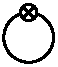
\includegraphics{frg/diagrams/FRG-wetterichEq-FS0_1_1.pdf}\end{gathered}
			\end{align*}
	\item<2-|handout:1> Exakte funktionale Differentialgleichung \textbf{aber} zur expliziten Lösung sind Trunkierungen nötig!
	\end{itemize}
	
	\blfootnote{%
		\fncitec{Wilson:1971bg,Wilson:1971dh,Wilson:1979qg}{Wilson 1971, Wilson 1979} und \fncitec{\frgWetterichEq}{Wetterich 1993, Reuter und Wetterich 1994, Morris 1994, Tetradis und
	Wetterich 1994, Ellwanger 1994}%
	}
	
	\note{
		\begin{itemize}
			\item Die funktionale Renormierungsgruppe (kurz) FRG ist eine dieser funktionalen Methoden.
			\item Die grundlegende Idee der FRG ist das \textbf{Ausintegrieren von Quantenfluktuationen} Impulsschale für Impulsschale nach Wilson.
			\item In der FRG interpoliert man mit einem \textbf{geeigneten Skalen abhängigem Funktional} -- hier groß Gamma:
			\item \textbf{zwischen der mikroskopischen, klassischen Wirkung bei hohen RG-Impuls-Skalen im UV}
			\item \textbf{zu einer makroskopischen Quanten Wirkung bei verschwindenden RG-Impulsskalen-Skalen im IR.} \switch
			\item Diese \textbf{Skalenevolution ist durch die Wetterich Gleichung in Form einer exakten, funktionale Differential Gleichung} beschrieben. Hier formuliert als eine Evolutionsgleichung in \textbf{RG Zeit}. Die RG Zeit $t$ ist eine \textbf{dimensionslose logarithmische Parametrisierung} der RG-Impuls-Skala $k$ \textbf{und wir evolvieren damit von $t=0$ im UV nach $t$ gegen $\infty$ im IR.} \switch
			\item \textbf{Explizite Lösungen der vollen funktionalen Differentialgleichungen lassen sich jedoch im Allgemeinen nicht berechnen.}
			\item \textbf{Für praktische Rechnungen sind Problem- und Theorie-spezifische Trunkierungen und Näherungen nötig.}
		\end{itemize}
	}
\end{frame}

\begin{frame}{Forschungsprojekte im Rahmen der Dissertation}
	\vspace{-0.1cm}
	\begin{itemize}
		\item<1-|handout:1> \textbf{Problem:} Etablierte Diskretisierungsverfahren für trunkierte FRG Flussgleichungen sind numerisch unzuverlässig für
		\begin{itemize}
			\item Stark im Feldraum gekoppelte Probleme mit Phasenübergängen
			\item Probleme mit intern/externen getriebenen Schocks/Diskontinuitäten
			\item Anwendungen bei kleinen $T$, $k$ und besonders bei hohem $\mu$
		\end{itemize}\vspace{0.25em}
		\item<2-|handout:1> \textbf{Lösung:} Reformulierung der Flussgleichungen in konservativer Form $\Rightarrow$ Behandlung im Rahmen der Strömungsmechanik\vspace{0.6em}
		\item<3-|handout:1> \textbf{Adaption von Konzepten und numerischen Methoden aus dem Feld der Strömungsmechanik auf FRG Flussgleichungen}
		\item<3-|handout:1> \textbf{Einfluss von bosonischen und fermionischen Fluktuationen auf homogene und inhomogene chirale Kondensate}
	\end{itemize}
	
	\uncover<3-|handout:1>{\tikz[overlay, remember picture]{
		%\draw[gray, thin, step=1cm] (current page.south west) grid (current page.north east);  % Draw a grid over the slide
		\draw[rounded corners, thick,goetheBlau] (0., 2.8) rectangle (11, 0.55);
		\node[align=left,anchor=east, font=\normalsize, text=goetheBlau] at (11.14, 0.27) {\textbf{Zentrale Forschungsprojekte}};
	}}

	\blfootnote{%
		\fnciteay{Grossi:2019urj}, \fnciteay{zerod1,zerod2,zerod3} und \fnciteay{gn,gns}%
	}
	
	\note{
		\begin{itemize}
			\item Ein großes Problem, welches im Rahmen unserer Forschung auftrat, war jedoch das etablierte Lösungsverfahren für tunkierte Flussgleichungen sich als unzuverlässig erwiesen haben. Zumindest für die Art von Fragestellungen hier an denen wir interessiert sind.\switch
			\item Kollegen aus Heidelberg haben damals die Lösung angestoßen. Diese besteht in einer Reformulierung von Flussgleichungen in konservativer Form.
			Dies wiederum erlaubt die direkte Anwendung von \textbf{hoch-entwickelten numerischen Methoden aus dem Feld der Strömungsmechanik}.\switch
			\item Es haben sich damit \textbf{zwei zentrale Forschungsprojekte} im Rahmen meiner Promotion gebildet. 
			\item Zum Einen\textbf{ methodische Entwicklungen zur Adaption von Konzepten aus der Strömungsmechanik auf FRG Flussgleichungen}. 
			\item Und zum Anderen, die \textbf{Anwendung dieser Methoden zum Studium von homogenen und inhomogenen chiralen Kondensaten}.
			Hierbei lag der \textbf{ Fokus auf dem Einfluss von fermionischen und bosonischen Fluktuationen}.
		\end{itemize}
	}
\end{frame}

\begin{frame}{Das \only<1|handout:0>{$O(N)$}\only<2>{$O(1)$}-Modell in \dimcomp{0} -- Die perfekte Testumgebung}
	Untersuchung von gewöhnlichen \only<1>{$N$-dimensionalen}\only<2>{eindimensionalen} Integralen der Form
		\only<1|handout:0>{
			\begin{align*}
				Z(\vec{J}\,) = \vphantom{\int_{-\infty}^{+\infty} }\int_{\Reals{}^N} \dif\vec{\phi}\, \exp\big(- \mathcal{S} ( \vec{\phi}\, )  +\vec{J}\cdot\vec{\phi}\,\big)
			\end{align*}
		}%
		\only<2>{
			\begin{align*}
				Z(J\,) = \int_{-\infty}^{+\infty} \dif\phi\, \exp\big(- \mathcal{S} ( \phi )  +J \phi \,\big)
			\end{align*}
		}%
	mit der Funktionalen Renormierungsgruppe:

	\begin{itemize}
		\item \textbf{Perfekte Testumgebung:} 
		\begin{itemize}
			\item Exakte Referenzwerte für alle Theorien \only<1|handout:0>{$\mathcal{S}(\vec{\phi}\,)$ mit $O(N)$ Symmetrie}\only<2>{$\mathcal{S}(\phi)$ mit $\mathbb{Z}_2$ Symmetrie}
			\item Keine Trunkierung nötig
			\item FRG Flussgleichungen: nicht-trivial und strukturell ähnlich zu $d>0$
			\item Ideal für konzeptionelle und numerische Entwicklungen
		\end{itemize}
	\end{itemize}

	\blfootnote{ \fnciteay{Keitel:2011pn} und \fnciteay{zerod1,zerod2,zerod3}}
	
	\note{
		\begin{itemize}
			\item Für die angesprochenen \textbf{technischen Entwicklungen haben wir null-dimensionale $O(N)$ Modelle verwendet}.
			\item Ein nulldimensionales $O(N)$-Modell ist ein sehr einfaches mathematisches Objekt: nämlich ein $N$-dimensionales, gewöhnliches Integral.
			Im Grenzfall für nur eine Skalar hier noch expliziter als ein eindimensionales Integral. \switch
			\item \textbf{Diese Art von Integral können wir für beliebige $\mathcal{S}$ und $J$ ganz einfach numerisch berechnen.}
			Wir können sie aber auch \textbf{alternativ mit exakten, nicht-trivialen FRG Flussgleichungen} lösen.
			\textbf{Exakte Flussgleichungen und exakte Referenzwerte machen null-dimensionale Modelle zur idealen Testumgebung.}
		\end{itemize}
	}
\end{frame}

\begin{frame}{Die FRG als Integraldeformation für $N=1$ mit $r(t)\equiv \Lambda\mkern1.5mu \eu^{-t}$}
	\centering
	\includegraphics[width=0.47\framewidth]{../0d/figures/rg_flow_integrand_z_smooth.pdf}
	
	\blfootnote{\fnciteay{zerod1}}
	
	\note{
		\begin{itemize}
			\item In \textbf{null Dimensionen } kann ich Ihnen jetzt auch \textbf{anschaulich erklären was die FRG jetzt eigentlich ist} und wie wir mit Ihr Integrale berechnen.
			\item \textbf{Mit der FRG Lösen wir Integrale in dem wir sie verformen.}
			\item Wir deformieren die komplizierten Integranden, die wir im IR berechnen wollen durch einen skalenabhänigen Massenterm auf einfache Glockenkurven im UV.
			\item Die Integrale im UV lassen sich dann einfach als Gauß'sche Integrale berechnen.
			\item Wir nehmen diese einfachen Integrale als Anfangsbedingung im UV und berechnen die komplizieren Integrale im IR durch sukzessive Deformation der Anfangsbedingung.
		\end{itemize}
	}
\end{frame}


\begin{frame}{FRG und numerische Strömungsmechanik}
	\begin{itemize}
		\item<1-|handout:1>	 FRG Flussgleichung für das $O(N)$-Modell in \dimcomp{0} als \textbf{Erhaltungsgleichung}:
			\begin{align*}
				\partial_\sigma \partial_t U(t,\sigma) \equiv \partial_t u ( t, \sigma ) = -\partial_\sigma \textcolor{emoRot}{F [ t, \sigma, u ( t, \sigma ) ]} + \partial_\sigma \textcolor{goetheBlau}{ Q [ t, \partial_\sigma u ( t, \sigma ) ]}
			\end{align*}
	\item<2-|handout:1>	\textbf{FRG-Fluss} im wahrsten Sinne des Wortes:\\[-1.75em]
		\begin{align*}
			\text{\textcolor{emoRot}{\textbf{Advektion:~}}}\textcolor{emoRot}{F [ t, \sigma, u ( t, \sigma ) ]} = \, & - ( N - 1 )\, \frac{\tfrac{1}{2} \, \partial_t r ( t )}{r ( t ) + \frac{1}{\sigma} \, u ( t, \sigma )} \, = \frac{1}{2}\,\begin{gathered}\includegraphics{diagrams/SU2model0d-UFlow_00103_1.pdf}\end{gathered}
			\\[-0.5em]
			\text{\textcolor{goetheBlau}{\textbf{Diffusion:~}}}\textcolor{goetheBlau}{ Q [ t, \partial_\sigma u ( t, \sigma ) ]} = \, & \frac{\tfrac{1}{2} \, \partial_t r ( t )}{r ( t ) + \partial_\sigma u ( t, \sigma )} \, = \input{diagrams/SU2model0d-Uflow_00014_1.tex}
			\end{align*}\vspace{-1.6em}			
\item<2-|handout:1> Adaption eines \textit{``finite volume''} Verfahrens für die FRG Flussgleichung
		\end{itemize}

\blfootnote{ \fnciteay{Grossi:2019urj} und \fnciteay{zerod1} mit Adaption von \fnciteay{KTO2-0} }

	\note{
		\begin{itemize}
			\item Diese \textbf{Deformation} wird auf dem Level eines \textbf{Skalen abhängigen WW Potenzial} in der FRG durch eine \textbf{partielle Differentialgleichung}
		beschrieben.
			\item Wenn wir eine \textbf{Ableitung dieser Gleichung in Feldrichtung} betrachten finden wir eine \textbf{Erhaltungsgleichung}: eine Flussgleichungen im wahrsten Sinne. \switch
			\item Wir behandeln hier eine konservative Gleichung mit einem \textbf{Advektions- und einem Diffusionsterm}.\switch
			\item Für die numerische Lösung dieser Gleichungen haben wir ein,\textbf{ in der Strömungsmechanik fest etabliertes, \textit{finite volume} Verfahren adaptiert}.
		\end{itemize}
	}
\end{frame}

\begin{frame}{FRG Fluss für $N = 1$ und $\mathcal{S}(\phi)=U(t=0,\phi)=-\tfrac{1}{2}\phi^2+\tfrac{1}{4!}\phi^4$}
	\centering
	\includegraphics[width=0.47\framewidth]{../0d/figures/sc_ii_n_on=1_n=800_xmax=10_lambda=1.0e12_tir=60_rg_flow.pdf}

	\blfootnote{\fnciteay{zerod1}}

	\note{
		\begin{itemize}
			\item Damit nun die besprochene Integral Deformation als numerischer FRG Fluss: \textbf{oben der Fluss des Potentials} und \textbf{unten der zu Grunde liegende Fluss der Ableitung}.
			\item \textbf{Wir haben im UV bei $t=0$ die klassische, mikroskopische Wirkung als Anfangsbedienung und evolvieren diese in RG Zeit durch numerisches Lösen der Flussgleichungen ins IR zu hohen RG Zeiten und erhalten so die volle makroskopische Quantenwirkung.}
		\end{itemize}
	}
\end{frame}

\begin{frame}{Und noch viel mehr $\ldots$}
	\hypersetup{linkcolor=goetheBlauDarker} 
	\begin{itemize}
		\item \hyperlink{0dScII}{Weitere Testszenarien}
		\item \hyperlink{0dadvection}{Advektion vs. Diffusion -- Pionen vs. Sigma}
		\item \hyperlink{0dscaling}{Skalierungs- und Konvergenztests}
		\item \hyperlink{0dxmax}{Randbedingungen}
		\item \hyperlink{0dLambda}{RG-Konsistenz und UV Skalen $\Lambda$}
		\item \hyperlink{0dTaylor}{Vergleich mit Taylor-/Vertex-Entwicklung}
		\item \hyperlink{0dkrange}{Dynamische Reichweite und IR Cutoffs}
		\item \hyperlink{0dentropie}{Irreversibilität und ``Entropie''-Produktion}
		\item \hyperlink{0dlargeN}{Advektive Flüsse bei großem $N$}
		\item \hyperlink{0dfermion}{\textbf{Graßmann-Zahlen: ``Fermionen'' in null Dimensionen}}
	\end{itemize}

	\blfootnote{ \fnciteay{zerod1,zerod2,zerod3}}
	\note{
		\begin{itemize}
			\item \textbf{An dieser Stelle würde ich gerne viel mehr von unseren Entwicklungen in null Dimensionen präsentieren, aber dann würde mir die Zeit fehlen, die folgenden Anwendungen auf physikalische Modelle zu besprechen.}
		\end{itemize}
	}
\end{frame}

\section[GNY-Modell in \dimcomplus{1}{1}]{Gross-Neveu-Yukawa-Modell in \dimcomplus{1}{1}}

\begin{frame}{Gross-Neveu-Yukawa-Modell in \dimcomplus{1}{1}}
	\textbf{Testmodell in $1+1$ Dimensionen zum Studium von diskreter chiraler ($\mathbb{Z}_2$) Symmetriebrechung}
	\begin{align*}
		\bar{\Gamma}_t [\chi] = \, &\intx[x]\!\!\, \Big( \bar{\psi} \, \big( \slashed{\partial} - \mu \gamma^2 + \tfrac{h}{\sqrt{N}} \, \varphi \big) \, \psi - \tfrac{1}{2} \, \varphi \, ( \Box \varphi ) + U ( t, \varphi ) \Big)
	\end{align*}\vspace{-.5cm}
	\begin{itemize}
		\item $N$ über eine Yukawa-Kopplung ($h$) wechselwirkende Fermionen
		\item Asymptotisch frei und renormierbar
		\item $\ldots$
	\end{itemize}
	$\Rightarrow$ Gut geeignet für Untersuchungen verschiedener technischer -- für QCD Materie relevanter -- Aspekte.
	
	\blfootnote{\fnciteay{gn,gns}}
	
	\note{
		\begin{itemize}
			\item \textbf{Daher nun direkt von Null zu Zwei Dimensionen: Hier haben wir das sog. Gross-Neveu-Yukawa-Modell mit der FRG studiert. Dieses eignet sich sehr gut als Testmodell zum Studium von dynamischer chiraler Symmetriebrechung.}
			\item Dieser Mechanismus ist äußerst relevant für QCD.
		\end{itemize}
	}
\end{frame}

\begin{frame}{Trunkierte Flussgleichung in \textit{``local potential approximation''}}
	\begin{itemize}
		\item<all:+->	LPA Flussgleichung für das GNY-Modell in  \dimcomplus{1}{1}:
			\begin{align*}
				\partial_t \partial_\sigma U ( t, \sigma ) \equiv \partial_t u ( t, \sigma ) = \partial_\sigma \textcolor{goetheBlau}{ Q [ t, \partial_\sigma u ( t, \sigma ) ]} + \textcolor{gruen}{ S [ t, \sigma]}
			\end{align*}
		\item	\textbf{\textcolor{goetheBlau}{Diffusion}sgleichung mit \textcolor{gruen}{Quellen/Senken}:}\\[-1.25em]
			\begin{align*}
				\textcolor{goetheBlau}{ Q [ t, \partial_\sigma u ( t, \sigma ) ]} = \, & \input{diagrams/SU2model0d-Uflow_00014_1.tex}
				=\,  - \frac{1}{\piu N} \, \frac{k_t^3}{2 E_{\textrm{b}} ( t, \partial_\sigma u )} \, \big[ 1 + 2 \, n_\mathrm{b} ( \beta E_{\textrm{b}} ( t, \partial_\sigma u ) ) \big]\\[.2cm]
				\textcolor{gruen}{S [ t, \sigma ]} =\,&-\frac{1}{2}\partial_\sigma \,\begin{gathered}
\includegraphics{diagrams/SU2model0d-UFlow_10002_1.pdf}\end{gathered}
				=\, \partial_\sigma  \bigg( \frac{1}{\piu} \, \frac{k_t^3}{E_{\textrm{f}} ( t, \sigma )} \, \big[ 1 -\\&\qquad - n_\mathrm{f} ( \beta [ E_{\textrm{f}} ( t, \sigma ) + \mu ] ) - n_\mathrm{f} ( \beta [ E_{\textrm{f}} ( t, \sigma ) - \mu ] ) \big] \bigg)
			\end{align*}\vspace{.2cm}
			mit $E_\mathrm{b} ( t, \partial_\sigma u ) \equiv \,  \sqrt{ k_t^2 + \partial_\sigma^2 U ( t, \sigma ) }$ und $E_\mathrm{f} ( t, \sigma ) \equiv \,  \sqrt{ k_t^2 + ( h \, \sigma )^2 }$.
	\end{itemize}
	
	\blfootnote{\fnciteay{gn}}
	
	\note{
		\begin{itemize}
			\item Lassen Sie mich\textbf{ direkt zur Flussgleichungen} kommen. In der sogenannten local potential approximation kurz LPA manifestiert sich die Flussgleichung wieder als Erhaltungsgleichung.
			Diesmal als eine Diffusionsgleichung mit Quellen und Senken. 
			\item \textbf{Hier liefert das Boson den diffusen Beitrag und die Fermionen sind für die Quellen und Senken verantwortlich.}
		\item \textbf{Auf diese Gleichung können wir im Prinzip direkt die in null Dimensionen entwickelten Konzepte anwenden.}
		\end{itemize}
	}
\end{frame}

\begin{frame}{FRG Flüsse im GNY-Modell}
	\begin{columns}
		\begin{column}{0.47\framewidth}
			\centering
			nur fermionische Fluktuationen (MF: $N\rightarrow\infty$)\\\vspace{.2cm}
			\includegraphics[width=0.47\framewidth]{../gn/figures/flow_MF_T=0.00625,mu=0.6.pdf}
		\end{column}\hspace{.5cm}
		%
		\uncover<2-|handout:1>{\begin{column}{0.47\framewidth}
			\centering
			fermionische und bosonische Fluktuationen (LPA: $N=2$)\\\vspace{.2cm}
			 \includegraphics[width=0.47\framewidth]{../gn/figures/flow_N=2,T=0.00625,mu=0.6.pdf}
		\end{column}}
	\end{columns}
	
	\blfootnote{\fnciteay{gn}}
	\note{
		\begin{itemize}
			\item \textbf{Hier ein exemplarischer FRG Fluss zunächst nur unter Berücksichtigung der Fermionen.} Wir
			starten im \textbf{UV mit einer freien Theorie }und fließen ins IR. Dabei agieren die \textbf{Fermionen auf
			Level des Potenzials als Senken} und es bildet sich ein \textbf{nicht triviales Minimum}.
			Dieses \textbf{Minimum signalisiert eine spontane chirale Symmetriebrechung} welche dynamisch durch das Ausintegrieren der fermionischen Fluktuationen ermöglicht wird.
			Es bildet sich als Konsequenz ein \textbf{nichtverschwindendes chirales Kondensat} aus. \switch
			\item \textbf{Betrachten wir nun rechts die Rolle von bosonsichen Fluktuationen}. \textbf{Zunächst dominieren wieder die Fermionen} und es bildet sich ein Minimum aber auf Grund der \textbf{Diffusion durch die bosonischen Fluktuationen} überlebt dieses nicht bis ins IR.
			Im \textbf{IR ist die chirale Symmetrie nicht mehr spontan gebrochen}.
			\textbf{Sprich die Bosonen verdampfen das durch die Fermionen gebildete chirale Kondensat.}
		\end{itemize}
	}
\end{frame}

\begin{frame}{Das homogene Phasendiagramm}
	\hypersetup{linkcolor=goetheBlauDarker} 
	\begin{columns}
		\begin{column}{0.47\framewidth}
			\centering
			\includegraphics[width=0.47\framewidth]{../gn/figures/phase_boundaries.pdf}
		\end{column}\hspace{.1cm}
		%
		\begin{column}{0.5\framewidth}
			\begin{itemize}
				\item Keine Symmetriebrechung im IR für endliche $N$ und $T>0$
				\item \hyperlink{2dvac}{Symmetriebrechung im Vakuum ($T=\mu=0$)}
				\item \hyperlink{2dqpt}{Anzeichen für Symmetriebrechung bei $T=0$ und $\mu>0$}
			\end{itemize}
		\end{column}
	\end{columns}

	\blfootnote{\fnciteay{gn}}
	
	\note{
		\begin{itemize}
			\item \textbf{Derartige Flüsse können wir nun bei verschiedenen Temperaturen und chemischen Potenzialen berechnen und so ein Phasendiagramm ermitteln.}
			\item\textbf{Generell haben unsere Untersuchungen gezeigt, dass das chirale Kondensat mit sinkender RG Skala immer weiter schrumpft und letztlich im IR für nicht-verschwindende Temperaturen komplett von den Bosonen verdampft wird.}
			\item \textbf{Nur bei verschwindenden Temperaturen finden wir Anzeichen für Kondensation.}
			\item \textbf{Mit formal undenklich vielen Fermionen lassen sich die bosonischen Fluktuationen komplett unterdrücken und wir reproduzieren das bekannte Literaturergebnis (hier links in Gelb) mit einer gebrochenen Phase bei niedrigen Temperaturen und chemischen Potentialen und einer Restaurierten Phase bei höheren.}
			\item \textbf{Das Literaturergebnis ohne bosonische Fluktuationen in der sog. Mean-Field Näherung basiert jedoch auf der restriktiven Annahme, dass das chirale Kondensat homogen in der einen Raumrichtung des Modells vorliegt.}
		\end{itemize}
	}
\end{frame}

\begin{frame}{Inhomogene Phasen im MF/Limes $N\rightarrow\infty$}
	\includegraphics[width=0.47\framewidth]{../gn/figures/largeN_pd.pdf}\hspace{.5cm}
	\includegraphics[width=0.47\framewidth]{../gn/figures/condensate.pdf}
	
	\uncover<2-|handout:1>{
	\begin{itemize}
		\item Semi-analytische Methoden zur direkten Berechnung einer inhomogenen Phase (IP) für $N\rightarrow\infty$
		\item Stabilitätsanalyse als flexible indirekte Detektionsmethode
	\end{itemize}
	}
	
	\blfootnote{Literaturergebnisse \fnciteay{Schnetz:2004vr,Schnetz:2005ih,Schnetz:2005vh,Basar:2009fg} und Stabilitätsanalyse \fnciteay{gns}}
	
	\note{
		\begin{itemize}
			\item Arbeiten die ein \textbf{inhomogenen Kondensat zulassen} finden zwar auch eine \textbf{homogen-gebrochene Phase} hier, aber bei höheren chemischen Potenzialen und entsprechenden Dichten findet man eine\textbf{ äußerst dominante inhomogene Phase} hier.
			In dieser Phase oszilliert das Kondensat wie hier links veranschaulicht im Raum.
			Bei hohen Temperaturen finden wir dann wieder die homogen restaurierte Phase. \switch
		\item \textbf{Dieses Literatur Ergebnis wurde mit äußerst speziellen und komplizierten semi-analytischen Methoden berechnet, welche sich nicht direkt vom MF auf die FRG übertragen lassen.}
			\item \textbf{Daher haben wir dieses Modell zur Hand genommen um eine Stabilitätsanalyse der homogenen Phase als alternative und flexiblere Methode im Detail zu testen.}
		\end{itemize}
	}
\end{frame}

\begin{frame}{Stabilitätsanalyse der homogenen Phase im MF/Limes $N\rightarrow\infty$}
	\hypersetup{linkcolor=goetheBlauDarker} 
	\begin{columns}
		\begin{column}{0.47\framewidth}
			\centering
			\includegraphics[width=0.47\framewidth]{../gn/figures/stab_pd.pdf}
		\end{column}\hspace{.1cm}
		%
		\begin{column}{0.5\framewidth}
			\begin{itemize}
				\item LP und (SP$\leftrightarrow$IP)-Phasengrenze sind mit der Stabilitätsanalyse \hyperlink{2dstab}{detektierbar}
				\item (HBP$\leftrightarrow$IP)-Phasengrenze \hyperlink{2dstab}{nicht detektierbar}
				\item \textit{``Moat regime''} mit $Z<0$ als Vorläufer der inhomogenen Phase
			\end{itemize}
		\end{column}
	\end{columns}

	\blfootnote{\fnciteay{gns} und Arbeiten zum \textit{``Moat regime''} \fnciteay{Rennecke:2021ovl,Pisarski:2020gkx,Pisarski:2021qof, Pisarski:2020dnx}}
	
	\note{
		\begin{itemize}
			\item \textbf{Mit dieser indirekten Methode ist man in der Lage eine inhomogene Phase und dessen Vorläufer zu finden und auch gewisse quantitative Aussagen sind möglich.}
		\end{itemize}
	}
\end{frame}

\section[QM-Modell in \dimcomplus{3}{1}]{Quark-Meson-Modell in \dimcomplus{3}{1}}

\begin{frame}{Zwei Flavor Quark-Meson-Modell in \dimcomplus{3}{1}}
	\textbf{Effektive Niederenergietheorie der QCD im Rahmen der FRG hier wieder in LPA} 
		\begin{align*}
			\FSeaa_k[\chi]&= \intx[x]\!\,\Big( 
			\bar{\psi}\big(\gamma_\mu \partial_\mu -\gamma_4\mu + h( \suIItup{0}\MFphi_0 + \iu\gammach \suIItup{a}\MFphi_a )\big)\psi 
			+\tfrac{1}{2}\big(\partial_\mu\MFphi\big)^2
			+U_{k}(\tfrac{\MFphi^2}{2})
			\Big)
		\end{align*}\vspace{-.5cm}
		\begin{itemize}
			\item Explizites inhomogenes Kondensat: chirale Dichtewelle (CDW)
			\begin{align*}
				\MFphi(\vec{x}\vts)\equiv (\sigma(\vec{x}\vts),0,0,\pi_3(\vec{x}\vts)) \equiv \Delta(\cos(\vec{q}\cdot\vec{x}\vts),0,0,\sin(\vec{q}\cdot\vec{x}\vts))
			\end{align*}
			\item Analytische Konstruktion der \textbf{\hyperlink{cdwFlow}{expliziten LPA Flussgleichung der CDW}} mittels {\hypersetup{linkcolor=goetheBlauDarker}\hyperlink{cdwU}{unitärer Transformationen}}
		\end{itemize}

	\blfootnote{\fnciteay{FuQCDRev}, \fnciteay{Dautry:1979bk} und \fnciteay{Steil:2024phd}}
	
	\note{
		\begin{itemize}
			\item Damit möchte ich zum Abschluss kurz zu meinen \textbf{Rechnungen in vier Dimensionen} kommen. Hier habe ich das\textbf{ Quark-Meson-Modell als effektive Niederenergietheorie der QCD} studiert.
			\item \textbf{Das Ziel hier ist explizite inhomogene chirale Phasen in einem QCD nahen Modell im Rahmen der FRG zu studieren. Diese Untersuchung dient als komplementäre Rechnung zu existierenden und geplanten Stabilitätsanalysen.}
			\item \textbf{Ich habe in local potential approximation ein sehr spezielles inhomogenes Kondensat betrachtet. Und zwar die sog. chirale Dichtewelle in der das Kondensat zwischen einer Pion und Sigma Richtung spiralförmig im Raum rotiert.}
			\item \textbf{Diese Art von Kondensat hat eine Vielzahl mathematisch angenehmer Eigenschaften, welche es mir ermöglicht haben eine explizite Flussgleichung abzuleiten.}
		\end{itemize}
	}
\end{frame}

\begin{frame}{Das inhomogene Phasendiagramm in MF}
	\textbf{RG-konsistente MF Rechnungen -- nur fermionische Fluktuationen -- als erster Schritt zur vollen Lösung und als Konsistenzcheck zu existierenden MF Rechnungen}\\\vspace{.4cm}
	\centering
	\includegraphics[width=0.7\framewidth]{../qmm/figures/eMFA_QMMCDW_PD_BC_04_all_88_300_600.pdf}
	
	\blfootnote{Existierenden MF Rechnungen \fnciteay{Adhikari:2017ydi,Carignano:2014jla}}
	
	\note{
		\begin{itemize}
			\item Mit der hergeleiteten Flussgleichungen habe ich zunächst \textbf{MF Rechnungen unter Vernachlässigung der bosonischen Fluktuationen }angestellt.
			Diese Rechnungen dienen als \textbf{erster Schritt hin zu einer vollständigen Lösung }und ermöglicht als \textbf{Konsistenzcheck einen Vergleich mit MF Literaturergebnissen}.
			\item Wie für \textbf{rein fermionischen Rechnungen} in dieser Art von Modellen üblich, findet man auch mit der FRG als Regularisierung, eine \textbf{inhomogene Phase — hier in diesem schmalen Streifen}.
		\end{itemize}
	}
\end{frame}

\section{Zusammenfassung und Ausblick}

\begin{frame}{Zusammenfassung}
	\begin{itemize}
		\item (Numerische) Strömungsmechanik für die FRG
		\begin{itemize}
			\item Methodische, konzeptionelle und didaktische Entwicklungen in \dimcomp{0}
			\item Anwendung im Gross-Neveu-Yukawa-Modell: Bosonische Fluktuationen verhindern Kondensation bei $T\neq 0$ in \dimcomplus{1}{1}
		\end{itemize}\vspace{0.2em}
		\item Stabilitätsanalyse als indirekte Detektionsmethode für inhomogene Phasen\vspace{0.2em}
		\item Quark-Meson-Modell mit explizitem inhomogenen Kondensat im Rahmen der FRG
		\begin{itemize}
			\item FRG Flussgleichung für CDW Kondensat mittels unitärer Transformationen
			\item RG-konsistente MF Rechnung als erster Schritt zur vollen numerischen Lösung
		\end{itemize}
	\end{itemize}
	
	\blfootnote{\fnciteay{zerod1,zerod2,zerod3}, \fnciteay{gn} und \fnciteay{gns}}
	
	\note{
		\begin{itemize}
			\item \textbf{Damit bin ich quasi am Ende meines Vortrags angelangt. Lassen sie mich kurz Zusammenfassen:}
			\item Ich habe mich im Rahmen meiner Promotion mit numerischer Strömungsmechanik für FRG Flussgleichungen beschäftigt
			\item und homogene und inhomogene chirale Kondensate in zwei und vier dimensionalen Modellen untersucht.
		\end{itemize}
	}
\end{frame}

\begin{frame}{Ausblick}
	\begin{itemize}
		\item (Numerische) Strömungsmechanik für die FRG in \dimcomp{0}
		\begin{itemize}
			\item \textbf{Modelle mit Graßmann-Zahlen} $\Rightarrow$ Laufende Yukawa Kopplung
			\item Entropie Funktion in Anwesenheit von Quelltermen
		\end{itemize}\vspace{0.2em}
		\item Gross-Neveu-Yukawa-Modell in \dimcomplus{1}{1}
		\begin{itemize}
			\item Stabilitätsanalyse mit bosonischen Fluktuationen
			\item Verbesserung der Trunkierung
		\end{itemize}\vspace{0.2em}
		\item Quark-Meson-Modell in \dimcomplus{3}{1}
		\begin{itemize}
			\item \textbf{Veröffentlichung der RG-konsistenten MF Rechnung und Flussgleichung mit der CDW}
			\item \textbf{Numerische Lösung der hergeleiteten Flussgleichung für die CDW $\Rightarrow$ Einfluss von bosonischen Fluktuationen auf explizites inhomogenes Kondensat}
			\item Komplementäre Stabilitätsanalyse $\Rightarrow$ Direkte vs. indirekte Detektion inhomogener Phasen
		\end{itemize}
	\end{itemize}

	\blfootnote{\fncitec{Steil:partIVminimal}{Steil und Koenigstein (in Vorbereitung)} und \fncitec{Steil:2024RGMF}{Steil, Buballa und Schaefer (in Vorbereitung)}}
	
	\note{
		
		\begin{itemize}
			\item \textbf{Abschließen will ich letztlich mit diesem Ausblick über geplante und mögliche weiterführende Forschung.}
			\item In Bezug auf\textbf{ Null dimensionale Modelle } sind \textbf{Grassmann-Zahlen als das Analogon zu Fermionen in null Dimensionen} noch ein großer Forschungsschwerpunkt.\textbf{ Hier haben wir ein Manuskript in Arbeit.}
			\item \textbf{Im Gross-Neveu-Yukawa-Modell gibt es auch noch vielversprechende und wichtige Weiterentwicklungen aber mein Fokus liegt aktuell auf den begonnen Arbeiten im Quark-Meson-Modell.}
			\item Hier steht die \textbf{Veröffentlichung der MF Rechnungen und Flussgleichungen für die CDW} noch aus. \textbf{Auch hierzu ist ein Manuskript in Arbeit.}
			\item \textbf{Der logische nächste große Schritt ist dann die volle Lösung der hergeleiteten Flussgleichungen mit den nun etablierten numerischen Methoden.}
		\end{itemize}\vspace{1em}
		\begin{itemize}
			\item \textbf{Damit bin ich am Ende meines Vortrags angelangt und ich Danke vielmals für Ihre Aufmerksamkeit!}
		\end{itemize}
	}
\end{frame}

% Black slide using TikZ
{
\usebackgroundtemplate{
\tikz[overlay,remember picture] \fill[deepblack] (current page.south west) rectangle (current page.north east);
}
\begin{frame}[plain,noframenumbering]
\end{frame}
}

\appendix
\begin{backup}

\section{Referenzen}
\setbeamertemplate{frametitle continuation}{}
\begin{frame}[allowframebreaks]{Referenzen}
	\begingroup
		\printbibliography[heading=none]
	\endgroup
\end{frame}

\section{Weitere Ergebnisse und Plots für \dimcomp{0}}

{\hypersetup{linkcolor=white} 
\begin{frame}{Testszenario I: \hyperlink{0dxmax}{Nicht stetiges Potential}}
\label{0dScII}
	\centering
	\includegraphics[width=0.47\framewidth]{../0d/figures/rg_flow_integrand_z_kink.pdf}\hspace{.5cm}
	\includegraphics[width=0.47\framewidth]{../0d/figures/sc_i_on=1_n=800_xmax=10_lambda=1.0e6_tir=60_rg_flow.pdf}
\end{frame}
}

\begin{frame}{Advektion vs. Diffusion -- Pionen vs. Sigma}
	\label{0dadvection}
	\centering
	\includegraphics[width=0.38\framewidth]{../0d/figures/sc_i_on_1_10_100_n_800_xmax_10_lambda_1e6_tir_60_rg_flow.pdf}
\end{frame}

\begin{frame}{Räumlicher Diskretisierungsfehler für $	U ( \vec{\varphi} \vts ) = -\tfrac{1}{2} \, \vec{\varphi}^{\vts 2} + \tfrac{1}{4!} \, ( \vec{\varphi}^{\vts 2} )^2 $}
	\label{0dscaling}
	\centering
	\includegraphics[width=0.38\framewidth]{../0d/figures/sc_ii_n_on_4_xmax_10_lambda_1e12_tir_60_deltax_scaling.pdf} 
\end{frame}

\begin{frame}{Berechnungsintervall für Testszenario I}
\label{0dxmax}
	\centering
	\begin{align*}
		U ( \vec{\varphi} \vts ) =
		\begin{cases}
			- \tfrac{1}{2} \, \vec{\varphi}^{\vts 2} \, ,			&	\text{if} \quad |\vec{\varphi}| \leq 2 \, ,\\
			- 2 \, ,									&	\text{if} \quad 2 < |\vec{\varphi}| \leq 3 \, ,\\
			+ \tfrac{1}{2} \, ( \vec{\varphi}^{\vts 2} - 13 ) \, ,	&	\text{if} \quad 3 < |\vec{\varphi}| 
		\end{cases}
	\end{align*}\vspace{0.5cm}\\
	\includegraphics[width=0.47\framewidth]{../0d/figures/sc_i_on_1_deltax_25e-3_lambda_1e6_tir_60_errors_xmax.pdf}\hspace{.5cm}
	\includegraphics[width=0.47\framewidth]{../0d/figures/sc_i_on_3_deltax_25e-3_lambda_1e6_tir_60_errors_xmax.pdf} 
\end{frame}


\begin{frame}{RG-Konsistenz und UV-Skalen $\Lambda$ für Testfall I}
	\label{0dLambda}
	\centering
	\includegraphics[width=0.6\framewidth]{../0d/figures/sc_i_on_3_n_400_xmax_10_rir_10e-20_cutoff_test.pdf}
\end{frame}


\begin{frame}{FRG Taylor-/Vertex-Expansion fürr $	U ( \vec{\varphi} \vts ) = \mp\tfrac{1}{2} \, \vec{\varphi}^{\vts 2} + \tfrac{1}{4!} \, ( \vec{\varphi}^{\vts 2} )^2 $}
	\label{0dTaylor}
	\centering
	\includegraphics[width=0.47\framewidth]{../0d/figures/sc_ii_n_on_4_lambda_1e12_tir_60_vertex_exp_error.pdf}\hspace{.5cm}
	\includegraphics[width=0.47\framewidth]{../0d/figures/sc_ii_p_on_4_lambda_1e12_tir_60_vertex_exp_error.pdf} 
\end{frame}


\begin{frame}{Dynamische-Reichweite und IR Cutoffs für Testfall I}
	\label{0dkrange}
	\centering
	\includegraphics[width=0.47\framewidth]{../0d/figures/sc_i_on_3_n_400_xmax_10_lambda_1e6_tir_60_mass_minimum.pdf}\hspace{.5cm}
	\includegraphics[width=0.47\framewidth]{../0d/figures/sc_i_on_3_n_400_xmax_10_lambda_1e6_tir_60_changing_rates.pdf} 
\end{frame}


\begin{frame}{Irreversibilität und ``Entropie''-Produktion für Testfall I}
	\label{0dentropie}
	\centering
	\includegraphics[width=0.47\framewidth]{../0d/figures/sc_i_on=1_n=800_xmax=10_lambda=1.0e6_tir=60_rg_flow.pdf}\hspace{.5cm}
	\includegraphics[width=0.47\framewidth]{../0d/figures/sc_i_on=1_n=800_xmax=10_lambda=1.0e6_tir=60_entropy_flow.pdf} 
\end{frame}


\begin{frame}{Irreversibilität und ``Entropie''-Produktion für Testfall II}
	\centering
	\includegraphics[width=0.47\framewidth]{../0d/figures/sc_ii_n_on=1_n=800_xmax=10_lambda=1.0e12_tir=60_rg_flow.pdf}\hspace{.5cm}
	\includegraphics[width=0.47\framewidth]{../0d/figures/sc_ii_n_on=1_n=800_xmax=10_lambda=1.0e12_tir=60_entropy_flow.pdf} 
\end{frame}


\begin{frame}{Flüsse bei $N\rightarrow\infty$ und $N=32$}
	\label{0dlargeN}
	\centering
	\includegraphics[width=0.36\framewidth]{../0d/figures/largeN_flows.pdf}\hspace{.5cm}
	\includegraphics[width=0.36\framewidth]{../0d/figures/N32_flows.pdf} 
\end{frame}



\begin{frame}{Ein \SU{2} Model -- stark gekoppelte Graßmannzahlen}
	\label{0dfermion}
	\centering

	\begin{align*}
		\FSeaa_\FSk[\MFchi]&=\del{\MFvtx{m}{\MFrho}\suIItij{0}{\alpha}{\beta}
		+\iu \MFvtx{h}{\MFrho}\suIItij{i}{\alpha}{\beta}\MFphi_i}\MFthetab_\alpha\MFtheta^\beta+\\
		&\qquad \qquad \qquad +\tfrac{1}{2}\MFvtx{g}{\MFrho}\suIItij{0}{\alpha}{\beta}\suIItij{0}{\delta}{\gamma}\MFthetab_\alpha\MFtheta^\beta\MFthetab_\delta\MFtheta^\gamma
		+ U_t(\MFrho)
	\end{align*}
\end{frame}

\section{Weitere Ergebnisse und Plots für \dimcomplus{1}{1} }

\begin{frame}{GNY Model im Vakuum mit $N=2$}
	\label{2dvac}
	\centering

	\includegraphics[width=0.47\framewidth]{../gn/figures/flow_L1D_N=2,T=0.0,mu=0.0.pdf}\hspace{.5cm}
	\includegraphics[width=0.47\framewidth]{../gn/figures/k_L1D_N=2,T=0.0,mu=0.0.pdf} 
\end{frame}

\begin{frame}{Restaurations-Skala $k_\mathrm{res}(T)$}
	\label{2dqpt}
	\begin{columns}
		\begin{column}{0.47\framewidth}  % This sets the width of the column to half the text width
			\centering
			\includegraphics[width=0.47\framewidth]{../gn/figures/T_k_restored.pdf} 
		\end{column}\hspace{.1cm}
		\begin{column}{0.5\framewidth}  % This also sets the width of the column to half the text width
			\begin{align*}
				k_\mathrm{res}(T)	\propto \begin{cases}
					T^0 &\text{für $\mu>0.6$,}\\
					T^1 &\text{für $\mu<0.6$}
				\end{cases}
			\end{align*}
		\end{column}
	\end{columns}
\end{frame}


\begin{frame}{Stabilitätsanalyse vs. semi-analytische Lösung}
	\label{2dstab}
	\centering
	\includegraphics[width=1.0\framewidth]{../gn/figures/q_stab_vs_min_muT.pdf}
\end{frame}

\section{Weitere Ergebnisse und Plots für \dimcomplus{3}{1} }

\begin{frame}{Unitäre Transformationen für die CDW}
\label{cdwU}
\textbf{Unitäre transformationen zur Diagonalisierung von $\FSvertexArg{\FSeaaEoMI}{\MFpsib, \MFpsi}$ und $\FSvertexArg{\FSeaaEoMI}{\MFphi_i, \MFphi_j}$:}

\begin{align*}
U_\psi(\vec{x}\vts)= \exp(- \iu \gammach t_3 \vec{q}\cdot\vec{x}\vts)
\end{align*}

\begin{align*}
U_\varphi(\vec{x}\vts)_{ij}=\frac{1}{2}\left(
\begin{array}{cccc}
	1 - \exp(-2\iu \vec q \cdot \vec x)& 0& 0& 1+\exp(-2\iu \vec q \cdot \vec x)\\
	0 & 2& 0&0\\
	0 & 0& 2&0\\
	-\iu(1+\exp(-2\iu \vec q \cdot \vec x)) & 0& 0& \iu(\exp(-2\iu \vec q \cdot \vec x)-1)\\
\end{array}
\right)_{ij}
\end{align*}
\end{frame}

\begin{frame}{Flussgleichung für QM Model mit CDW Kondensat}
	\label{cdwFlow}
	\hspace*{-1.5em}
	\begin{minipage}{\textwidth}
		\footnotesize\vspace{-0.15cm}
		\begin{align*}
			\partial_k U_k(\rho)&=12\int\! \frac{\dif^{\, 3}\!p}{(2\piu)^3}\sum_{\pm}\big[-1+\nf(\beta [E_{\psi;k}^\pm+\mu])+\nf(\beta [E_{\psi;k}^\pm-\mu])\big]\partial_k E_{\psi;k}^\pm+\notag\\[.1em]
			&\qquad\qquad\qquad\qquad\qquad +\int\! \frac{\dif^{\, 3}\!p}{(2\piu)^3}\sum_{i=0}^3\big(\tfrac{1}{2}+\nb(\beta E_{\phi,i;k})\big)\tilde{\partial}_k E_{\phi,i;k}
		\end{align*}\vspace{-0.4cm}

		\begin{align*}
			(E_{\psi;k}^\pm)^2&\stackrel{\phantom{q=0}}{=}M^2+\frac{(\vec{p}_k^{\mkern 2mu +q})^2}{2} +\frac{(\vec{p}_k^{\mkern 2mu -q})^2}{ 2}\pm\sqrt{M^2\del{\vec{p}_k^{\mkern 2mu +q}-\vec{p}_k^{\mkern 2mu -q}}^2+\frac{1}{4}\del{(\vec{p}_k^{\mkern 2mu +q})^2 -(\vec{p}_k^{\mkern 2mu -q})^2 }^2}\\
			&\stackrel{q=0}{=} M^2+\del{\vec{p}_k}^2
		\end{align*}\vspace{-0.4cm}
		\begin{align*}
			(E_{\phi;k}^{0,3})^2&\stackrel{\phantom{q=0}}{=}\frac{1}{2 }(\vec{p}_k)^2 +\frac{1}{2 }(\vec{p}_k^{\mkern 2mu+4q})^2+2U_k'(\rho) +2\rho U_k''(\rho)\,
			\pm \sqrt{4\rho^2 U_k''(\rho)^2+\frac{1}{4}\del{(\vec{p}_k^{\mkern 2mu+4q})^2-(\vec{p}_k)^2 }^2}\\
			&\stackrel{q=0}{=}\del{\vec{p}_k}^2+2U_k'(\rho)+2\rho (U_k''(\rho)\pm|U_k''(\rho)|)\\
			(E_{\phi;k}^{1})^2&=(E_{\phi;k}^{2})^2\stackrel{\phantom{q=0}}{=}(\vec{p}_k)^2+2U_k'(\rho)\stackrel{q=0}{=}\del{\vec{p}_k}^2+2U_k'(\rho)
		\end{align*}\vspace{-0.4cm}
		\begin{align*}
			\vec{p}_k^{\mkern 2mu q}&\equiv\del{\vec p + {\vec q/ 2}}\lambda_k\del{|\vec p + {\vec q/ 2}|}\qquad\text{und}\qquad
			M^2\equiv \frac{1}{4} h^2 \Delta^2=\frac{h^2}{2}\rho
		\end{align*}
	\end{minipage}
	
\end{frame}


\begin{frame}{Das Problem mit naiver Parameter-Fixierung}
	\begin{center}
		\begin{overlayarea}{\framewidth}{6.2cm}
				\only<1|handout:1>{\includegraphics[width=\framewidth]{figures/eMFAinhomo400.pdf}}
				\only<2|handout:2>{\includegraphics[width=\framewidth]{figures/eMFAinhomo450.pdf}}
				\only<3|handout:3>{\includegraphics[width=\framewidth]{figures/eMFAinhomo500.pdf}}
		\end{overlayarea}
	\end{center}
\end{frame}


\end{backup}
\end{document}
